% !TEX program = xelatex
\documentclass[aspectratio=169, 10pt]{beamer}

% ==========================
% GÓI NGÔN NGỮ & FONT (XELATEX / PDFLATEX)
% ==========================
\usepackage{iftex}
\ifPDFTeX
  \usepackage[utf8]{inputenc}
  \usepackage[vietnamese]{babel}
  \usepackage[T5,T1]{fontenc}
  \usepackage{lmodern}
\else
  \usepackage{fontspec}
  \setmainfont{DejaVu Sans}
  \setsansfont{DejaVu Sans}
\fi

\usepackage{amsmath, amssymb, amsfonts}
\usepackage{graphicx}
\usepackage{booktabs}
\usepackage{tabularx}
\usepackage{multirow}
\usepackage{colortbl}
\usepackage{tikz}
\usetikzlibrary{shapes.geometric, arrows, positioning, calc}

% Tự động fallback nếu đường dẫn ảnh bị thiếu
\let\origincludegraphics\includegraphics
\renewcommand{\includegraphics}[2][]{%
  \IfFileExists{#2}{%
    \origincludegraphics[#1]{#2}%
  }{%
    \IfFileExists{../CS231_tex_package_updated/#2}{%
      \origincludegraphics[#1]{../CS231_tex_package_updated/#2}%
    }{%
      \IfFileExists{../assets/#2}{%
        \origincludegraphics[#1]{../assets/#2}%
      }{%
        \fbox{\begin{minipage}[c][2.0cm][c]{0.7\linewidth}\centering\scriptsize\textcolor{red}{\textbf{[Chưa tìm thấy ảnh: \texttt{#2}]}}\end{minipage}}%
      }%
    }%
  }%
}

% ==========================
% BEAMER THEME & COLOR SCHEME (UIT BLUE STYLE)
% ==========================
\usetheme{Madrid}
\usecolortheme{default}

% Màu sắc nhận diện UIT & Báo cáo
\definecolor{uitblue}{RGB}{0, 85, 170}
\definecolor{uitdarkblue}{RGB}{0, 45, 110}
\definecolor{accentred}{RGB}{195, 30, 30}
\definecolor{softgreen}{RGB}{46, 125, 50}
\definecolor{cream}{RGB}{250, 248, 239}

\setbeamercolor{palette primary}{bg=uitblue,fg=white}
\setbeamercolor{palette secondary}{bg=uitdarkblue,fg=white}
\setbeamercolor{palette tertiary}{bg=uitdarkblue,fg=white}
\setbeamercolor{palette quaternary}{bg=uitblue,fg=white}
\setbeamercolor{structure}{fg=uitblue}
\setbeamercolor{titlelike}{parent=palette primary}
\setbeamercolor{frametitle}{bg=uitblue,fg=white}
\setbeamercolor{block title}{bg=uitblue,fg=white}
\setbeamercolor{block body}{bg=blue!5,fg=black}
\setbeamercolor{block title example}{bg=softgreen,fg=white}
\setbeamercolor{block body example}{bg=green!5,fg=black}
\setbeamercolor{block title alerted}{bg=accentred,fg=white}
\setbeamercolor{block body alerted}{bg=red!5,fg=black}

\setbeamertemplate{navigation symbols}{}
\setbeamertemplate{headline}{}

% Tùy biến Footline
\setbeamertemplate{footline}{
  \leavevmode%
  \hbox{%
  \begin{beamercolorbox}[wd=.333333\paperwidth,ht=2.25ex,dp=1ex,center]{author in head/foot}%
    \usebeamerfont{author in head/foot}CS231 -- Thị giác máy tính
  \end{beamercolorbox}%
  \begin{beamercolorbox}[wd=.333333\paperwidth,ht=2.25ex,dp=1ex,center]{title in head/foot}%
    \usebeamerfont{title in head/foot}Nhận dạng Biển báo Giao thông VN
  \end{beamercolorbox}%
  \begin{beamercolorbox}[wd=.333333\paperwidth,ht=2.25ex,dp=1ex,right]{date in head/foot}%
    \usebeamerfont{date in head/foot}\insertframenumber{} / \inserttotalframenumber\hspace*{2ex} 
  \end{beamercolorbox}}%
  \vskip0pt%
}

% ==========================
% THÔNG TIN TIÊU ĐỀ
% ==========================
\title[\textbf{Traffic Sign Recognition}]{\textbf{NHẬN DẠNG BIỂN BÁO GIAO THÔNG VIỆT NAM}}
\subtitle{\textbf{Two-Stage Hybrid Architecture: YOLO11s \& Enhanced LeNet-5 / SVM}}
\author[Tuấn Anh \& Thanh Tân]{\textbf{Sinh viên thực hiện:}\texorpdfstring{\\}{ }Từ Lê Tuấn Anh (24520133) -- Nguyễn Thanh Tân (24521581)}
\institute[UIT -- ĐHQG-HCM]{
  Khoa Khoa học Máy tính -- Trường Đại học Công nghệ Thông tin, ĐHQG-HCM\\[0.15cm]
  \textit{Môn học: Thị giác máy tính (CS231)}
}
\date{Học kỳ 1 -- Năm học 2026--2027}

% ==========================
% BẮT ĐẦU NỘI DUNG SLIDE
% ==========================
\begin{document}

% --------------------------
% SLIDE 1: TIÊU ĐỀ
% --------------------------
\begin{frame}[plain]
  \titlepage
\end{frame}

% --------------------------
% SLIDE 2: MỤC LỤC
% --------------------------
\begin{frame}{Nội dung báo cáo}
  \tableofcontents
\end{frame}

% ==========================================================
\section{Dẫn nhập \& Phát biểu bài toán}
% ==========================================================

% --------------------------
% SLIDE 3: DẪN NHẬP
% --------------------------
\begin{frame}{0. Dẫn nhập -- Bài toán từ góc nhìn camera hành trình}
  \begin{columns}[T]
    \begin{column}{0.52\textwidth}
      \textbf{Đặc thù giao thông Việt Nam:}
      \begin{itemize}\setlength{\itemsep}{1pt}\footnotesize
        \item \textbf{Đa dạng kích thước:} Cự ly xa $< 16 \times 16\text{ px}$, cự ly gần $> 100 \times 100\text{ px}$.
        \item \textbf{Biến thiên quang học:} Nắng gắt chói lóa, bóng râm, thiếu sáng ban đêm.
        \item \textbf{Nhiễu bối cảnh:} Bị tán cây, dây điện, xe cộ che khuất một phần.
        \item \textbf{Cùng màu khác hình:} Cùng xanh lam nhưng là hình tròn (Hiệu lệnh) hoặc chữ nhật (Chỉ dẫn).
      \end{itemize}
      \vspace{0.1cm}
      \begin{alertblock}{\scriptsize Mục tiêu nghiên cứu}
        \scriptsize Hệ thống phân loại chính xác cao, bền vững với ánh sáng, đạt thời gian thực ($\ge 300\text{ FPS}$) trên CPU.
      \end{alertblock}
    \end{column}
    \begin{column}{0.48\textwidth}
      \centering
      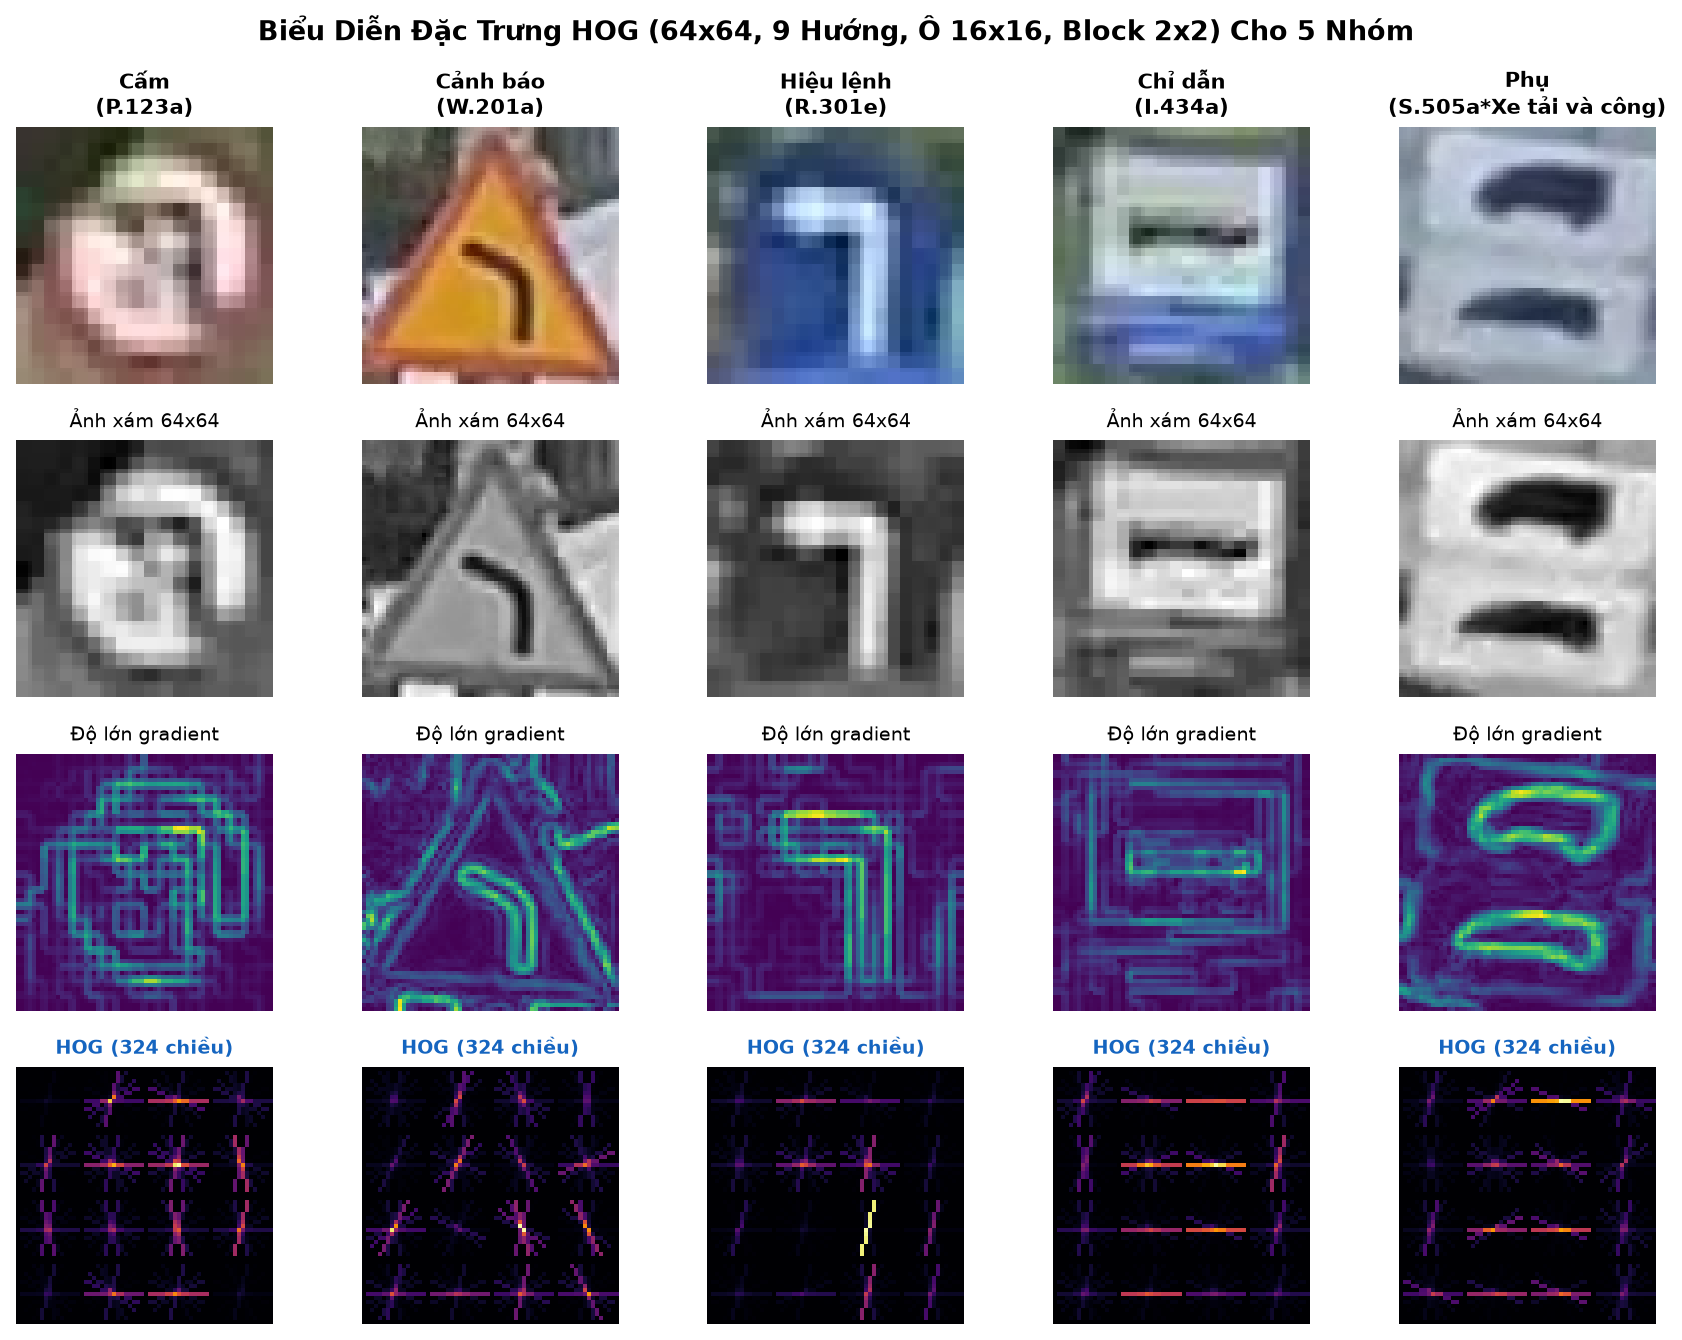
\includegraphics[width=0.92\linewidth]{graphics/sec3/f1_12_hog_visualization_groups.png}\\[0.1cm]
      \scriptsize \textit{4 nhóm quy chuẩn theo QCVN 41:2019/BGTVT}
    \end{column}
  \end{columns}
\end{frame}

% --------------------------
% SLIDE 4: PHÁT BIỂU BÀI TOÁN - CỐT LÕI
% --------------------------
\begin{frame}{1. Phát biểu bài toán -- Bài toán cốt lõi: Phân loại ảnh}
  \begin{block}{Input (Đầu vào)}
    \begin{enumerate}
      \item \textbf{Tập dữ liệu huấn luyện có nhãn:} $\mathcal{D} = \{(\mathbf{x}_i, y_i)\}_{i=1}^{N}$
      \begin{itemize}
        \item $\mathbf{x}_i \in \mathbb{R}^{h \times w \times 3}$: Ảnh vùng quan tâm (ROI crop) biển báo (hoặc vector $\mathbf{x}_i \in \mathbb{R}^{457}$).
        \item $y_i \in \mathcal{C}$: Nhãn chân lý (Ground truth) của ảnh thứ $i$.
      \end{itemize}
      \item \textbf{Ảnh biển báo cần dự đoán (Query image):} $\mathbf{x} \in \mathbb{R}^{h \times w \times 3}$
      \item \textbf{Tập các nhóm lớp quy chuẩn cho trước ($C = 4$):}
      $$\mathcal{C} = \{\text{Biển Cấm (P)}, \; \text{Biển Nguy Hiểm (W)}, \; \text{Biển Hiệu Lệnh (R)}, \; \text{Biển Chỉ Dẫn (I)}\}$$
    \end{enumerate}
  \end{block}

  \begin{exampleblock}{Output (Đầu ra)}
    \begin{itemize}
      \item Nhãn phân loại dự đoán $\hat{y} \in \mathcal{C}$ cùng độ tự tin $p \in [0, 1]$:
      $$\hat{y} = \arg\max_{c \in \mathcal{C}} P(y = c \mid \mathbf{x})$$
      \item \textbf{Mục tiêu:} Tối đa hóa Accuracy và Macro-F1 trên cả 4 nhóm lớp.
    \end{itemize}
  \end{exampleblock}
\end{frame}

% --------------------------
% SLIDE 5: VÍ DỤ MINH HỌA PHÂN LOẠI
% --------------------------
\begin{frame}{1. Phát biểu bài toán -- Ví dụ trực quan phân loại ảnh}
  \centering
  \textbf{Sơ đồ phân loại ảnh con (ROI Image Classification):}\\[0.1cm]
  \begin{tikzpicture}[
    node distance=0.8cm,
    box/.style={draw=uitblue, fill=blue!10, rounded corners=3pt, thick, align=center, inner sep=4pt, font=\scriptsize},
    arrow/.style={->, >=stealth, very thick, color=uitblue}
  ]
    \node[box] (input) {\textbf{Input}\\Ảnh ROI crop\\($64 \times 64 \times 3$)};
    \node[box, right=1.0cm of input, fill=cream, draw=accentred] (model) {\textbf{Bộ Phân loại}\\SVM (HOG + Color) /\\Enhanced LeNet-5};
    \node[box, right=1.0cm of model, fill=green!10, draw=softgreen] (output) {\textbf{Output}\\Nhãn $\hat{y} \in \mathcal{C}$\\Độ tin cậy $p$};

    \draw[arrow] (input) -- (model);
    \draw[arrow] (model) -- (output);
  \end{tikzpicture}

  \vspace{0.15cm}
  \begin{columns}[T]
    \begin{column}{0.48\textwidth}
      \centering
      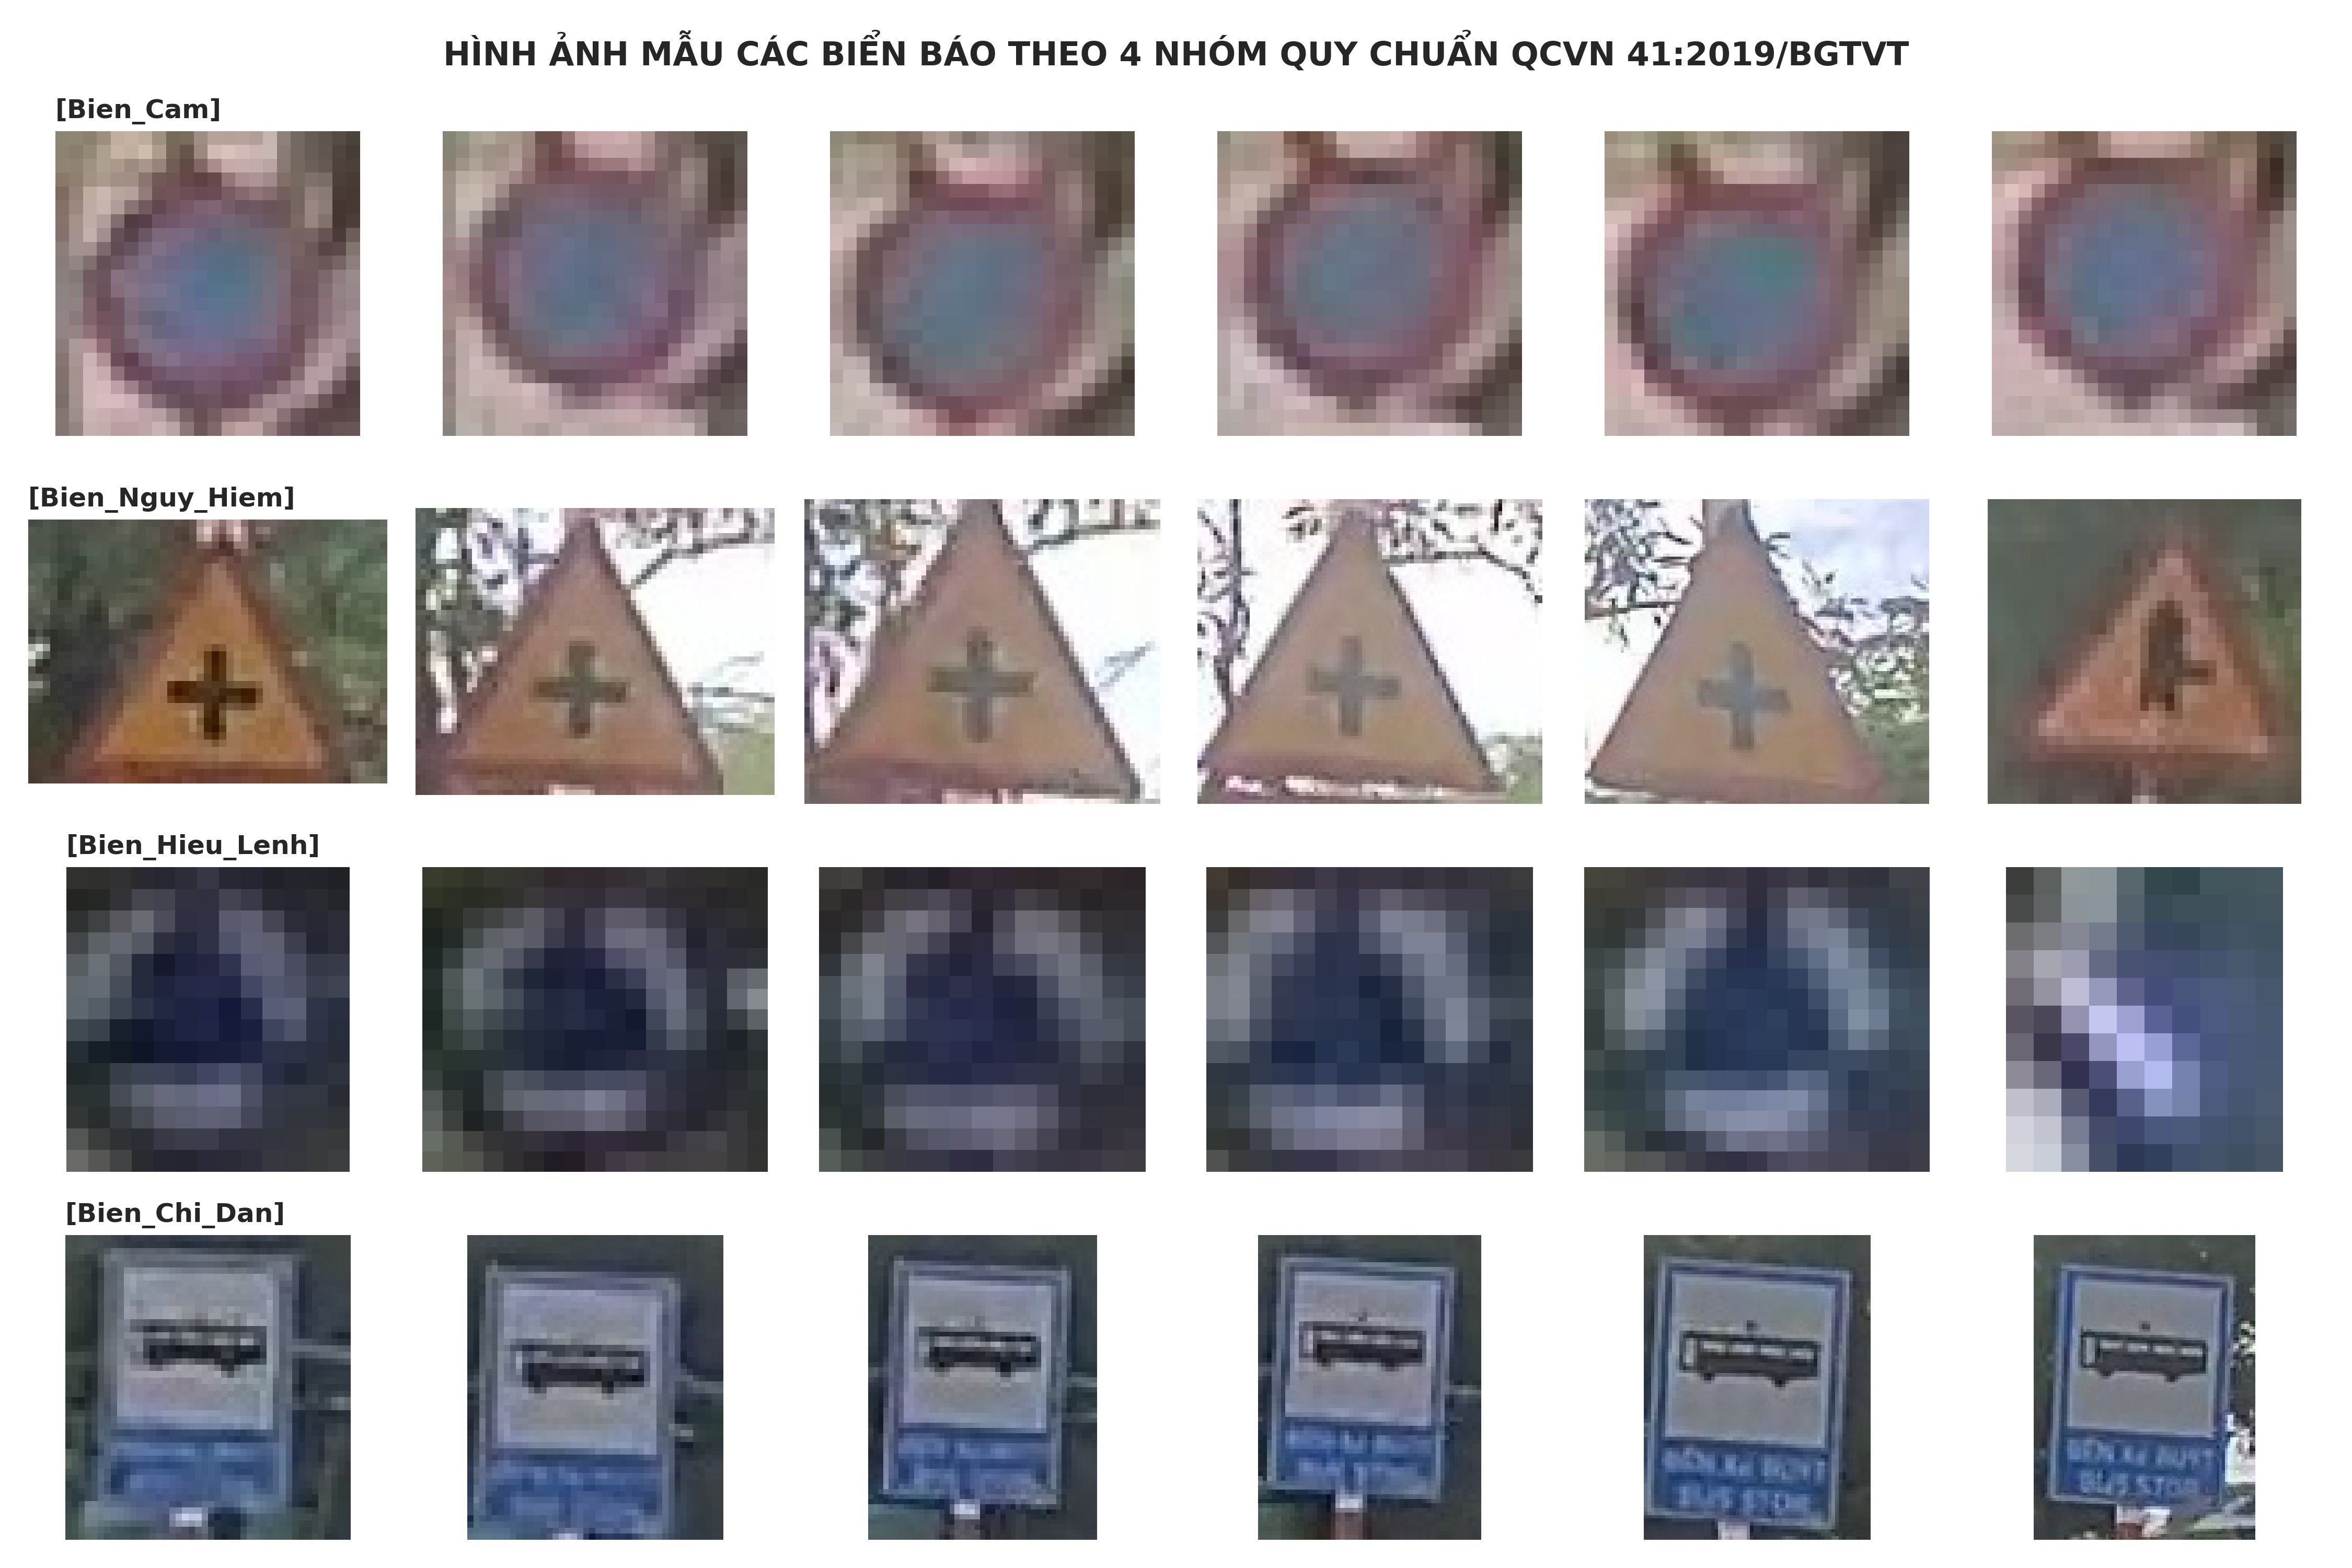
\includegraphics[width=0.95\linewidth]{graphics/eda/3_sample_traffic_signs_grid.png}\\[0.05cm]
      \scriptsize \textit{Các mẫu ảnh ROI trong tập dữ liệu Việt Nam}
    \end{column}

    \begin{column}{0.52\textwidth}
      \begin{block}{\textbf{Ví dụ phân loại thực tế}}
        \small
        \begin{itemize}\setlength{\itemsep}{2pt}
          \item \textbf{Biển Cấm (P.102):} Viền đỏ, nền trắng/gạch ngang\\$\rightarrow \hat{y} = \texttt{Bien\_Cam}$ ($p=0.99$) \textcolor{softgreen}{\textbf{[ĐÚNG]}}
          \item \textbf{Biển Chỉ Dẫn (I.407):} Nền xanh lam, hình vuông\\$\rightarrow \hat{y} = \texttt{Bien\_Chi\_Dan}$ ($p=0.97$) \textcolor{softgreen}{\textbf{[ĐÚNG]}}
          \item \textbf{Biển Nguy Hiểm (W.201):} Tam giác vàng viền đỏ\\$\rightarrow \hat{y} = \texttt{Bien\_Nguy\_Hiem}$ ($p=1.00$) \textcolor{softgreen}{\textbf{[ĐÚNG]}}
        \end{itemize}
      \end{block}
    \end{column}
  \end{columns}
\end{frame}

% --------------------------
% SLIDE 6: MỞ RỘNG TOÀN TRÌNH E2E
% --------------------------
\begin{frame}{1. Phát biểu bài toán -- Mở rộng: Pipeline nhận dạng toàn trình}
  \begin{alertblock}{Vấn đề thực tế}
    Camera hành trình thu nhận ảnh toàn cảnh đường phố ($1920 \times 1080$), biển báo chỉ chiếm $< 0.1\%$ diện tích canvas $\rightarrow$ Bắt buộc cần khâu Định vị tự động.
  \end{alertblock}

  \vspace{0.1cm}
  \begin{columns}[T]
    \begin{column}{0.65\textwidth}
      \textbf{Mô hình hóa hai giai đoạn (Two-Stage Decoupling):}
      \begin{enumerate}
        \item \textbf{Giai đoạn 1 (Localization -- YOLO11s 1-Class):}
        Quét toàn cảnh $\mathbf{I}$, xuất ra tập $K$ hộp bao:
        $$\mathcal{B} = \left\{ \hat{b}_k = (x_1, y_1, x_2, y_2)_k \;\middle|\; \text{conf}_k \ge 0.25 \right\}$$
        \item \textbf{Giai đoạn 2 (Classification -- Trọng tâm đề tài):}
        Cắt ảnh con $\mathbf{x}_k = \mathbf{I}[\hat{b}_k]$ đưa qua bộ phân loại để gán nhãn $\hat{y}_k \in \mathcal{C}$.
      \end{enumerate}
      \textbf{Output toàn trình:} $\hat{\mathcal{Y}} = \{(\hat{b}_k, \hat{y}_k, p_k)\}_{k=1}^K$
    \end{column}
    \begin{column}{0.35\textwidth}
      \centering
      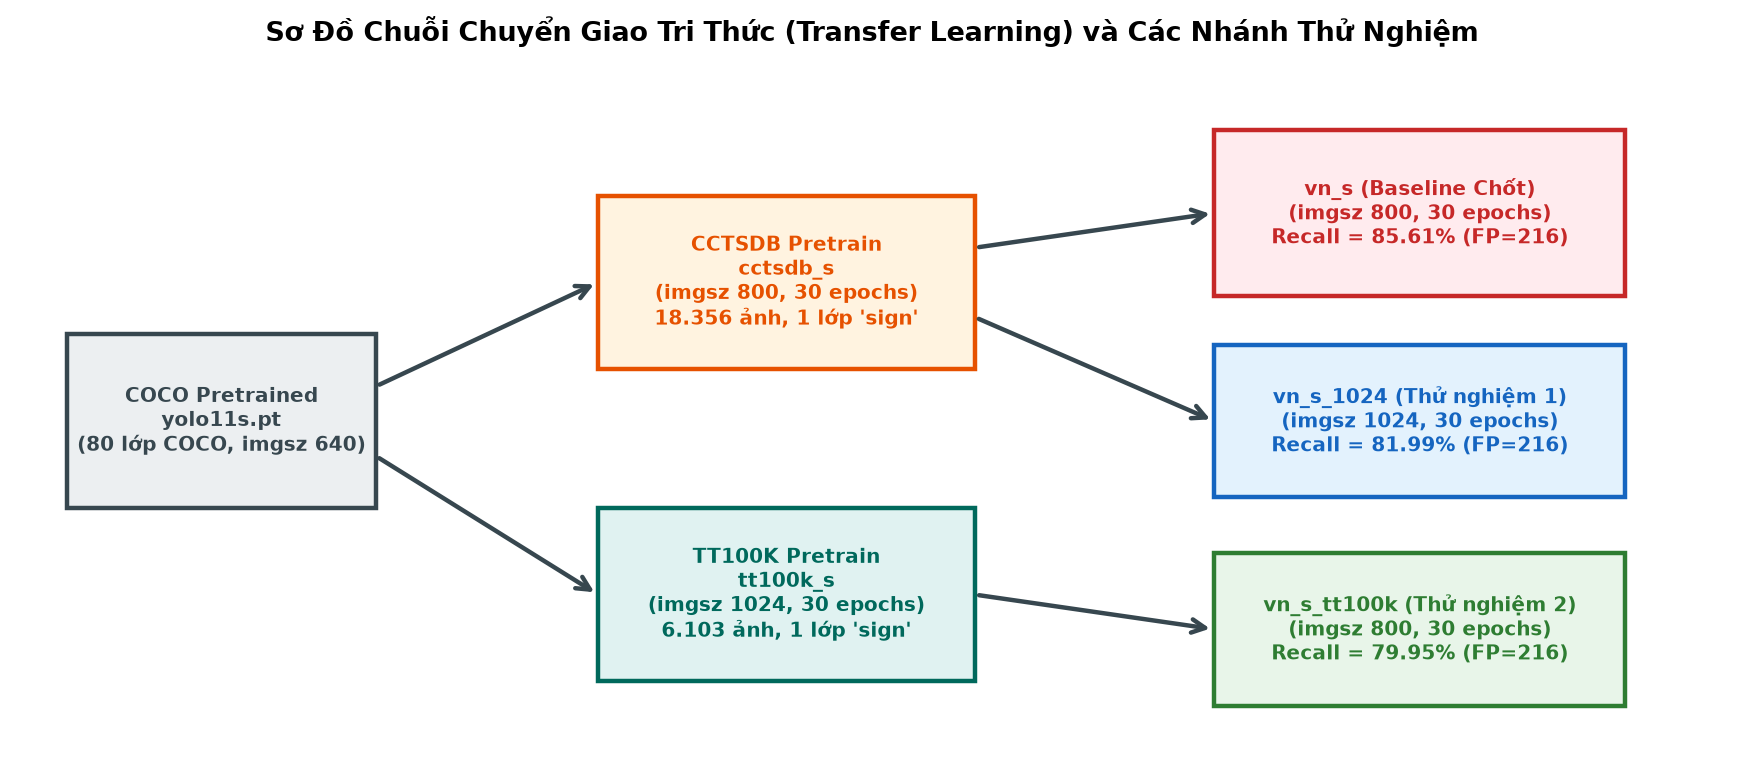
\includegraphics[width=\linewidth]{graphics/sec3/f2_01_transfer_learning_chain.png}\\[0.1cm]
      \scriptsize \textit{Chuỗi học chuyển giao tri thức}
    \end{column}
  \end{columns}
\end{frame}

% --------------------------
% SLIDE 7: CÁC GIAI ĐOẠN CHÍNH
% --------------------------
\begin{frame}{2. Các giai đoạn chính: Huấn luyện Offline \& Suy luận Online}
  \begin{columns}[T]
    \begin{column}{0.5\textwidth}
      \begin{block}{\textbf{Giai đoạn Huấn luyện (Offline)}}
        \textbf{1. Tiền huấn luyện \& Tinh chỉnh Detector:}
        \begin{itemize}
          \item Pretrain YOLO11s trên CCTSDB (17.856 ảnh) + 500 ảnh nền âm tính.
          \item Finetune trên dữ liệu Việt Nam (Train: 2.215 ảnh).
        \end{itemize}
        \textbf{2. Huấn luyện 2 nhánh Phân loại (5.401 ROI):}
        \begin{itemize}
          \item \textit{Nhánh Truyền thống:} Trích xuất HSV circular shift, Grid $2\times2$, HOG 457d $\rightarrow$ GridSearch RBF-SVM.
          \item \textit{Nhánh Học sâu:} Tăng cường dữ liệu (Augmentation), train Enhanced LeNet-5 qua 20 epochs (Adam + StepLR).
        \end{itemize}
      \end{block}
    \end{column}

    \begin{column}{0.5\textwidth}
      \begin{exampleblock}{\textbf{Giai đoạn Suy luận (Online Runtime)}}
        \begin{tikzpicture}[
          node distance=0.7cm,
          box/.style={draw=uitdarkblue, fill=white, rounded corners=3pt, thick, align=center, inner sep=4pt, font=\scriptsize},
          arr/.style={->, >=stealth, thick, color=uitdarkblue}
        ]
          \node[box] (in) {Khung hình Camera ($960 \times 540$ / $1080p$)};
          \node[box, below=of in] (det) {YOLO11s 1-Class ($\text{imgsz}=800$, conf $\ge 0.25$)};
          \node[box, below=of det] (crop) {Cắt các vùng ảnh con ROI ($\mathbf{x}_k$)};
          \node[box, below left=0.6cm and -0.4cm of crop, fill=cream] (svm) {Nhánh A: SVM RBF\\(2.63 ms/ảnh)};
          \node[box, below right=0.6cm and -0.4cm of crop, fill=blue!10] (cnn) {Nhánh B: LeNet-5\\(1.10 ms/ảnh)};
          \node[box, below=1.8cm of crop] (out) {\textbf{Xuất kết quả:} Hộp bao + Nhãn + Độ tin cậy};

          \draw[arr] (in) -- (det);
          \draw[arr] (det) -- (crop);
          \draw[arr] (crop) -| (svm);
          \draw[arr] (crop) -| (cnn);
          \draw[arr] (svm) |- (out);
          \draw[arr] (cnn) |- (out);
        \end{tikzpicture}
      \end{exampleblock}
    \end{column}
  \end{columns}
\end{frame}

% ==========================================================
\section{Phương pháp đề xuất \& Cấu hình kỹ thuật}
% ==========================================================

% ----------------------------------------------------------
% PHƯƠNG PHÁP 1: YOLO11s (1-CLASS DETECTOR)
% ----------------------------------------------------------

% SLIDE 8: TỔNG QUAN PHƯƠNG PHÁP YOLO11
\begin{frame}{3. Giai đoạn 1: Tổng quan phương pháp phát hiện đối tượng YOLO11}
  \begin{columns}[T]
    \begin{column}{0.56\textwidth}
      \begin{block}{\textbf{Nguyên lý Single-Stage Detector}}
        Phát hiện đối tượng trong \textbf{một lần quét (End-to-End)}, loại bỏ bước đề xuất vùng trượt tốn kém.
      \end{block}

      \textbf{Cấu trúc 3 thành phần chính của YOLO11:}
      \begin{itemize}\setlength{\itemsep}{1pt}\footnotesize
        \item \textbf{Backbone (C3k2):} Khối C3k2 cải tiến trích xuất đặc trưng đa quy mô với chi phí tính toán thấp.
        \item \textbf{Neck (PANet):} Hợp nhất đặc trưng ngữ nghĩa mức cao và chi tiết hình thái vật thể nhỏ.
        \item \textbf{Anchor-Free Head:} Dự đoán trực tiếp tọa độ tâm và kích thước hộp bao không cần anchor.
      \end{itemize}

      \textbf{Hàm mất mát:} $\mathcal{L}_{\text{YOLO}} = \lambda_{\text{box}} \mathcal{L}_{\text{CIoU/DFL}} + \lambda_{\text{cls}} \mathcal{L}_{\text{BCE}}$
    \end{column}

    \begin{column}{0.44\textwidth}
      \centering
      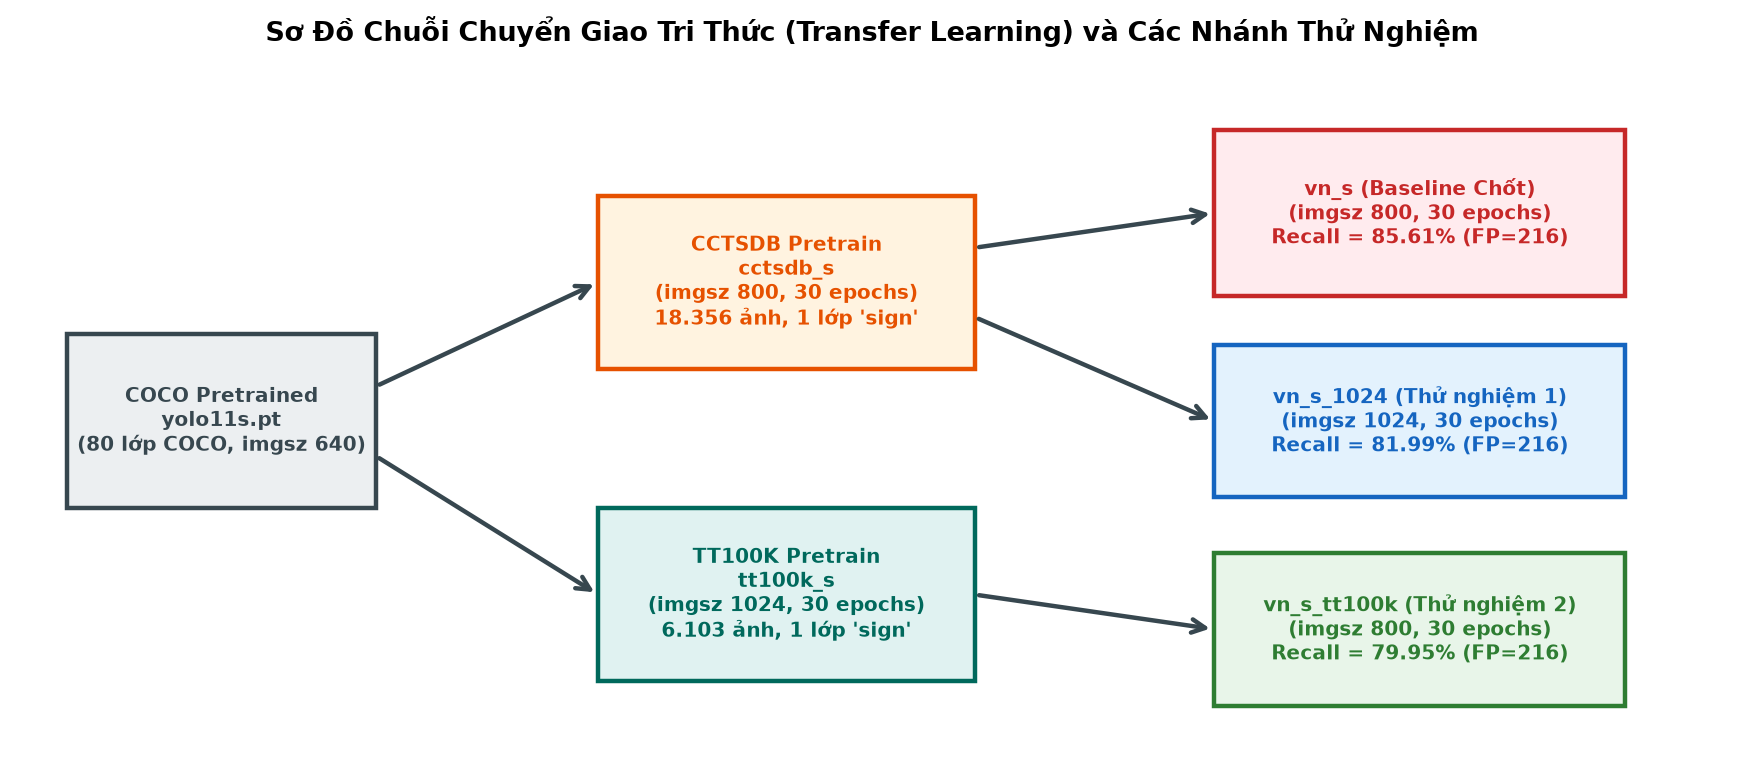
\includegraphics[width=0.92\linewidth]{graphics/sec3/f2_01_transfer_learning_chain.png}\\[0.1cm]
      \scriptsize \textit{Sơ đồ chuỗi chuyển giao đặc trưng YOLO11}
      \vspace{0.1cm}
      \begin{alertblock}{\scriptsize \textbf{Ưu thế công nghệ}}
        \scriptsize YOLO11 tối ưu hóa FLOPs, đạt tốc độ thời gian thực $> 70\text{ FPS}$ trên video camera hành trình.
      \end{alertblock}
    \end{column}
  \end{columns}
\end{frame}

% SLIDE 9: ÁP DỤNG YOLO11s VÀO BÀI TOÁN ĐỀ TÀI
\begin{frame}{3. Giai đoạn 1: Áp dụng YOLO11s vào bài toán định vị biển báo}
  \begin{columns}[T]
    \begin{column}{0.56\textwidth}
      \begin{block}{\textbf{Chiến lược chuyên biệt 1-Class (\texttt{"sign"})}}
        \footnotesize
        Biển báo ở xa chỉ chiếm $< 0.1\%$ diện tích canvas. Ép detector tập trung 100\% vào định vị $\rightarrow$ Tối đa hóa \textbf{Recall ($85.61\%$)}, không bỏ sót biển nguy hiểm.
      \end{block}

      \textbf{Cấu hình huấn luyện \& Vòng lặp (Training Loop):}
      \begin{itemize}\setlength{\itemsep}{1pt}\footnotesize
        \item \textbf{Pretrain:} 17.856 ảnh CCTSDB 2021 + 500 ảnh âm tính (Negative).
        \item \textbf{Finetune:} Dữ liệu Việt Nam, canvas $\text{\textbf{imgsz}} = \mathbf{800 \times 800}$.
        \item \textbf{Vòng lặp:} \textbf{30 epochs}, batch size $= 4$, SGD/AdamW ($\text{lr}_0 = 0.01$).
        \item \textbf{Augmentation:} Mosaic, Mixup, HSV jitter.
        \item \textbf{Ngưỡng suy luận Online:} $\tau_{\text{conf}} = 0.25$, $\text{NMS IoU} = 0.6$.
      \end{itemize}
    \end{column}

    \begin{column}{0.44\textwidth}
      \centering
      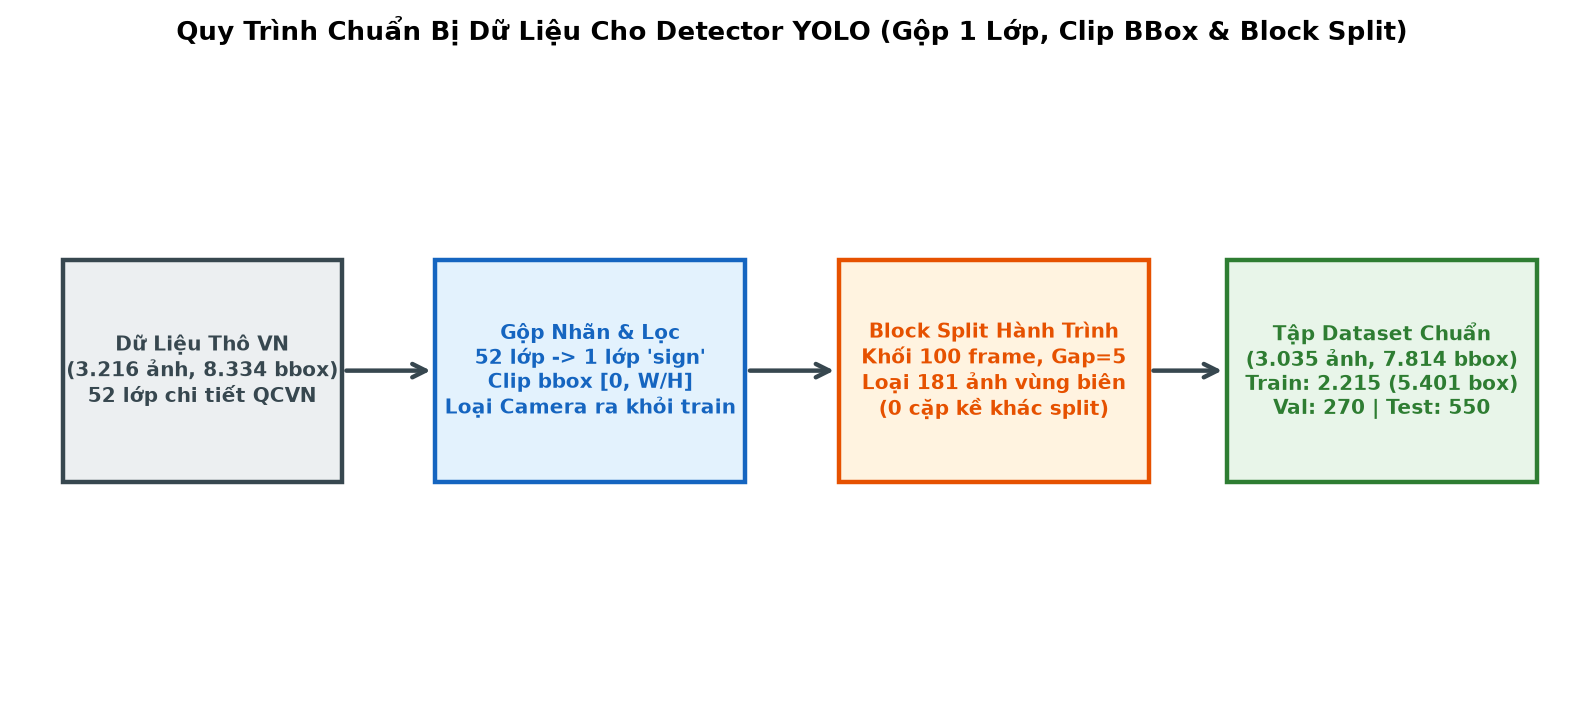
\includegraphics[width=0.92\linewidth]{graphics/sec3/f2_04_data_prep_flowchart.png}\\[0.1cm]
      \scriptsize \textit{Quy trình chuẩn bị dữ liệu \& tinh chỉnh YOLO11s}
      \vspace{0.1cm}
      \begin{exampleblock}{\scriptsize \textbf{Kết quả khâu Định vị}}
        \scriptsize Đạt \textbf{Detection Recall 85.61\%} và \textbf{mAP50 83.63\%}, tạo các crop ROI chuẩn xác cho khâu phân loại.
      \end{exampleblock}
    \end{column}
  \end{columns}
\end{frame}

% ----------------------------------------------------------
% PHƯƠNG PHÁP 2: THỊ GIÁC TRUYỀN THỐNG (COLOR + HOG + SVM)
% ----------------------------------------------------------

% SLIDE 10: TỔNG QUAN PHƯƠNG PHÁP HOG & SVM
\begin{frame}{3. Giai đoạn 2A: Tổng quan phương pháp HOG \& Máy học SVM}
  \begin{columns}[T]
    \begin{column}{0.55\textwidth}
      \begin{block}{\textbf{1. Đặc trưng HOG (Dalal \& Triggs, 2005)}}
        \footnotesize
        \begin{itemize}\setlength{\itemsep}{1pt}
          \item \textbf{Nguyên lý:} Hình dạng cục bộ được mô tả qua phân bố hướng gradient cường độ sáng.
          \item \textbf{Tính toán:} Sobel tính $G_x, G_y \rightarrow$ Biên độ $M$ và hướng $\theta \rightarrow$ Histogram 9 bins hướng / cell $\rightarrow$ Chuẩn hóa khối (Block $L_2$).
        \end{itemize}
      \end{block}

      \begin{exampleblock}{\textbf{2. Máy học SVM với hàm nhân RBF}}
        \footnotesize
        \begin{itemize}\setlength{\itemsep}{1pt}
          \item Cực đại hóa khoảng cách lề (Maximum Margin).
          \item Ánh xạ sang không gian Hilbert qua nhân RBF:
            $K(\mathbf{x}, \mathbf{x}') = \exp\left(-\gamma \|\mathbf{x} - \mathbf{x}'\|^2\right)$
        \end{itemize}
      \end{exampleblock}
    \end{column}

    \begin{column}{0.45\textwidth}
      \centering
      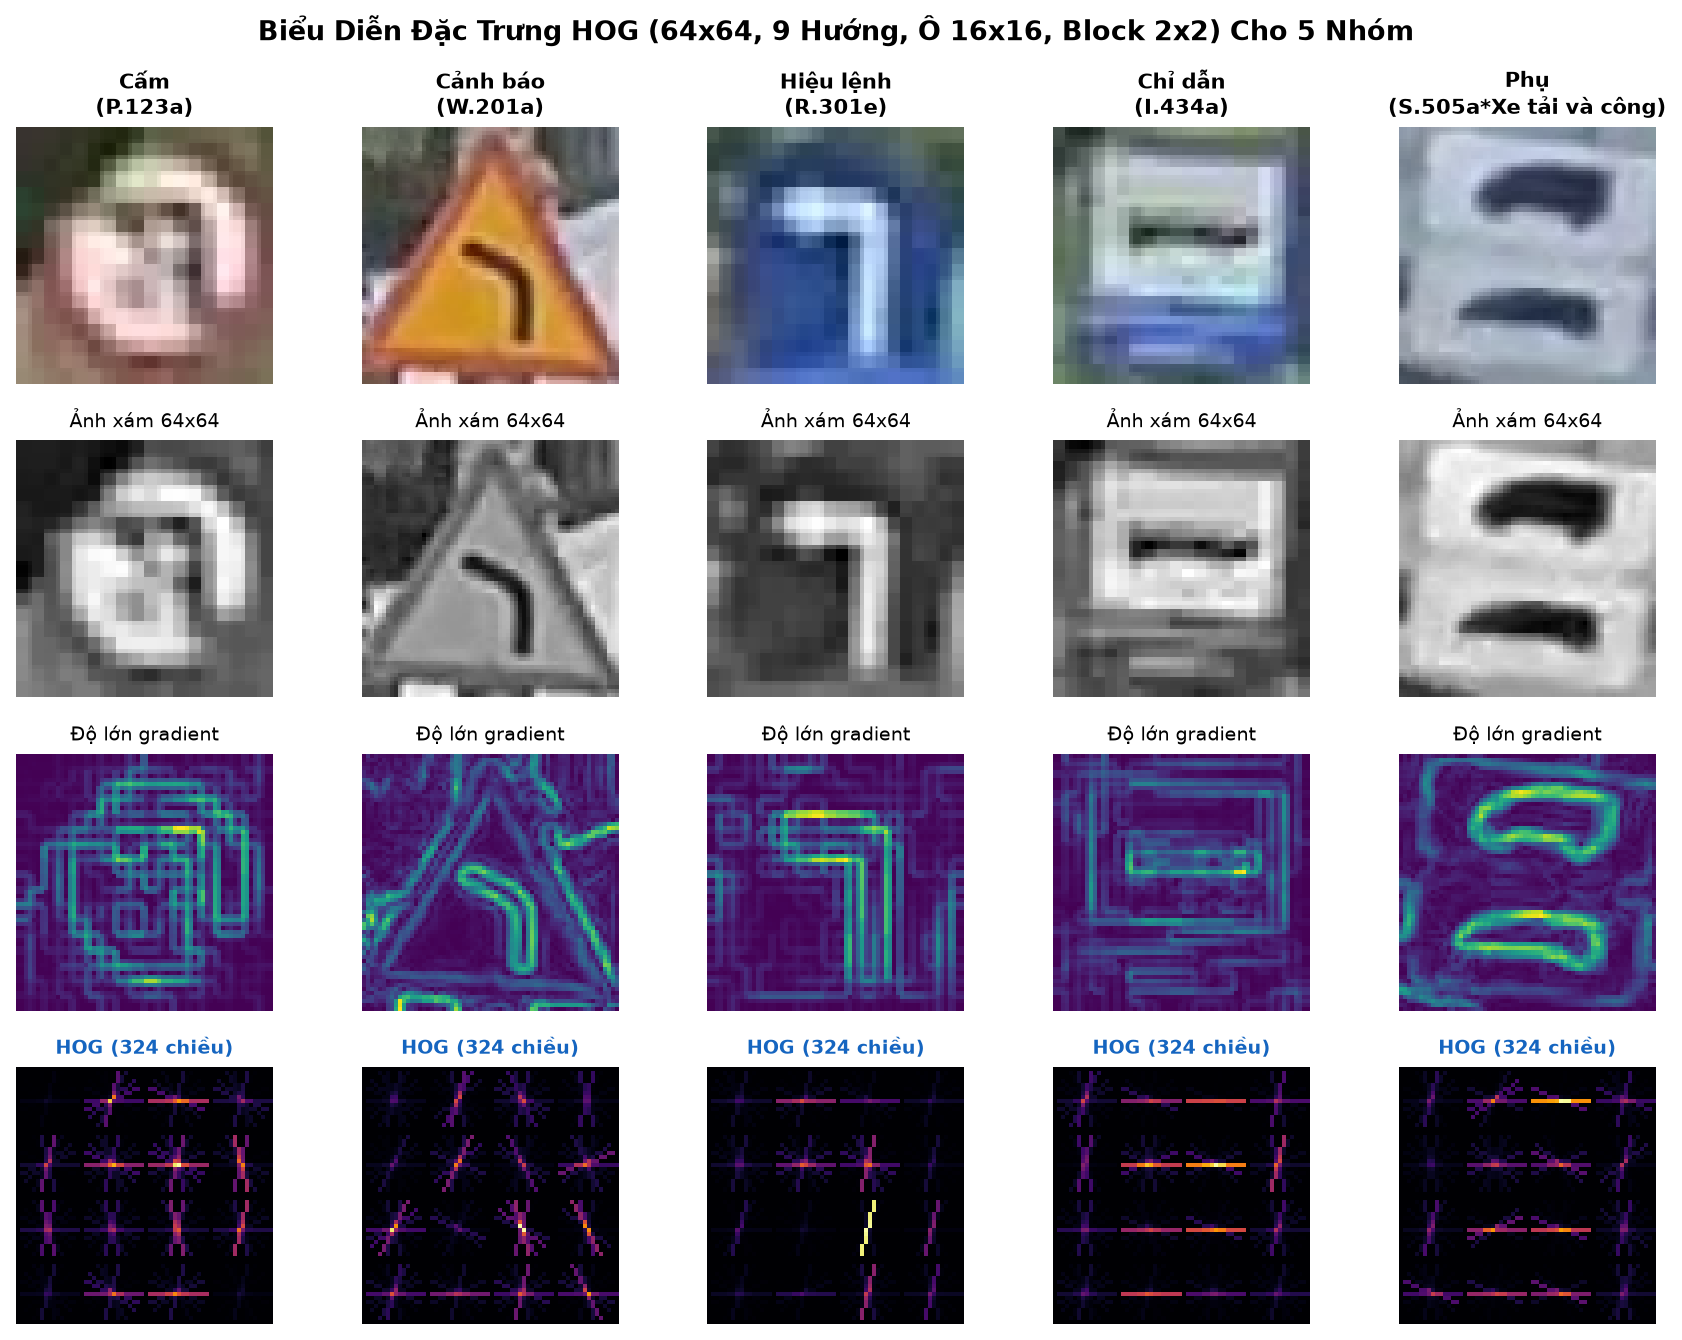
\includegraphics[width=0.90\linewidth]{graphics/sec3/f1_12_hog_visualization_groups.png}\\[0.1cm]
      \scriptsize \textit{Trực quan hóa vector HOG phân biệt 4 nhóm biển}
      \vspace{0.1cm}
      \begin{alertblock}{\scriptsize \textbf{Điểm mạnh HOG}}
        \scriptsize Bất biến với ánh sáng môi trường, bắt trọn viền tròn, tam giác, hình vuông.
      \end{alertblock}
    \end{column}
  \end{columns}
\end{frame}

% SLIDE 11: ÁP DỤNG HOG + HSV + SVM VÀO BÀI TOÁN
\begin{frame}{3. Giai đoạn 2A: Thiết kế đặc trưng S0--S3 \& Huấn luyện SVM}
  \begin{columns}[T]
    \begin{column}{0.56\textwidth}
      \textbf{Chuỗi ghép đặc trưng $\mathbf{s}_3 \in \mathbb{R}^{457}$ đa tầng (S0 $\rightarrow$ S3):}
      \begin{enumerate}\setlength{\itemsep}{1pt}\footnotesize
        \item \textbf{S0 (44d):} HSV dịch pha $(H+30)\pmod{180}$, \textbf{bỏ kênh V} (36 bin H + 8 bin S) $\rightarrow$ Miễn nhiễm chói nắng, bóng râm.
        \item \textbf{S1 (45d):} Tỷ lệ khung hình $\text{AR} = W_{\text{orig}}/H_{\text{orig}}$ trước khi resize.
        \item \textbf{S2 (133d):} Lưới không gian $2 \times 2$ (bắt viền đỏ và nền trong).
        \item \textbf{S3 (457d):} HOG trên \textbf{ảnh xám} ($64\times 64$, cell $16\times 16$, block $2\times 2$, 9 bins) $\rightarrow$ Thêm \textbf{324 chiều} gradient viền.
      \end{enumerate}

      \textbf{Cấu hình huấn luyện SVM (\texttt{sklearn.svm.SVC}):}
      \begin{itemize}\setlength{\itemsep}{1pt}\footnotesize
        \item Kernel: \textbf{RBF}, Tham số phạt $C = 5.0$, gamma $\gamma = \text{'scale'}$.
        \item Cân bằng mẫu: $\text{\texttt{class\_weight}} = \text{\texttt{'balanced'}}$ (chống lệch lớp).
        \item Tối ưu: Thuật toán SMO giải bài toán tối ưu lồi.
      \end{itemize}
    \end{column}

    \begin{column}{0.44\textwidth}
      \centering
      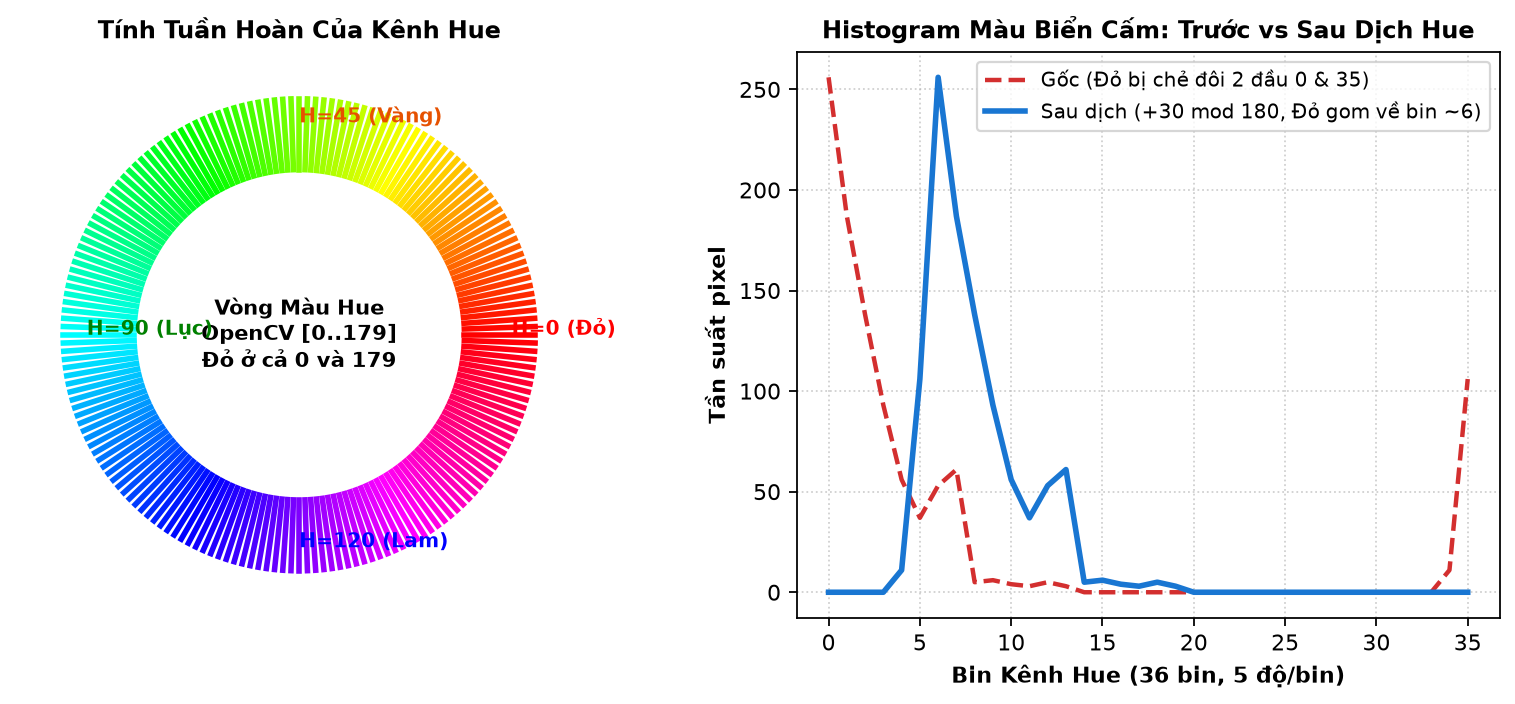
\includegraphics[width=0.78\linewidth]{graphics/sec3/f1_07_hue_circularity_shift.png}\\[0.05cm]
      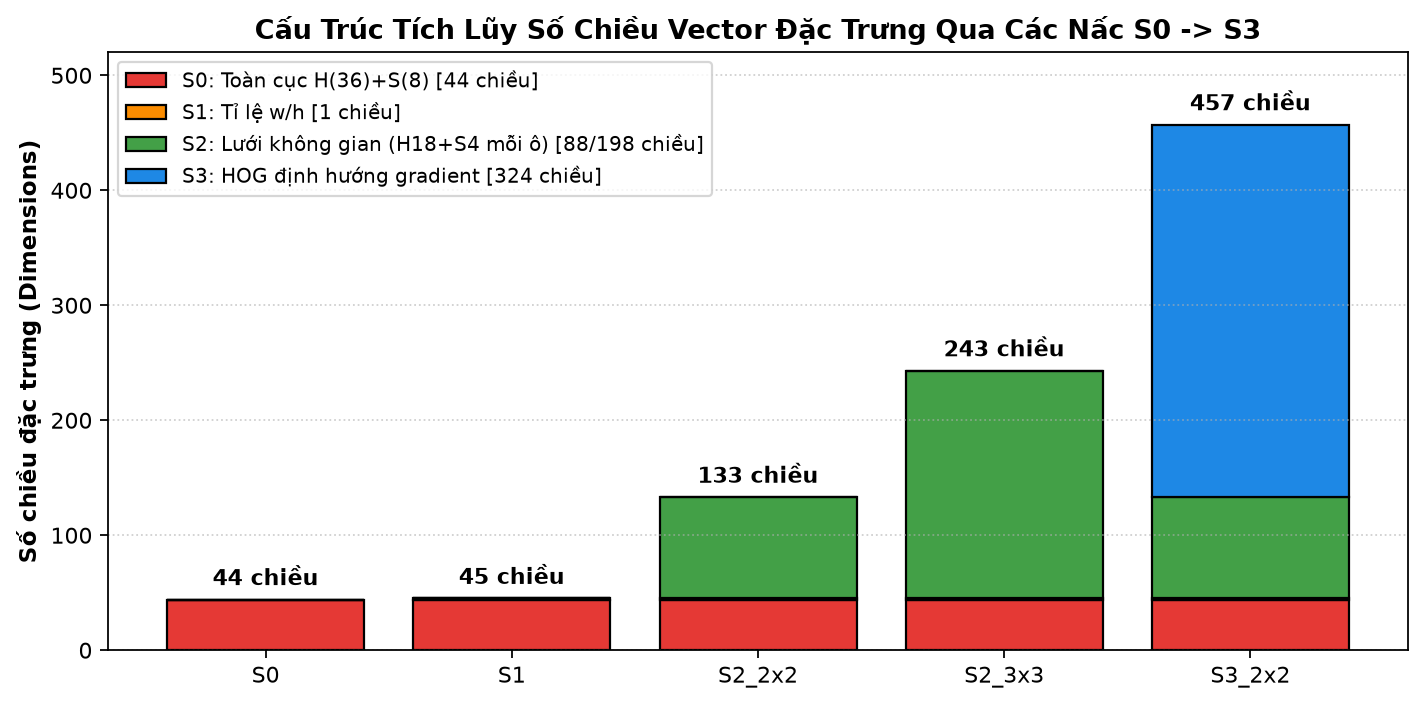
\includegraphics[width=0.78\linewidth]{graphics/sec3/f1_14_feature_vector_structure.png}\\[0.05cm]
      \scriptsize \textit{Dịch pha Hue \& Cấu trúc ghép vector 457 chiều}
    \end{column}
  \end{columns}
\end{frame}

% ----------------------------------------------------------
% PHƯƠNG PHÁP 3: HỌC SÂU HIỆN ĐẠI (ENHANCED LENET-5 CNN)
% ----------------------------------------------------------

% SLIDE 12: TỔNG QUAN PHƯƠNG PHÁP CNN & LENET-5
\begin{frame}{3. Giai đoạn 2B: Tổng quan Mạng nơ-ron tích chập (CNN) \& LeNet-5}
  \begin{columns}[T]
    \begin{column}{0.56\textwidth}
      \begin{block}{\textbf{Nguyên lý Mạng nơ-ron tích chập (CNN)}}
        \footnotesize
        \begin{itemize}\setlength{\itemsep}{1pt}
          \item \textbf{Conv Layer:} Quét kernel trích xuất đặc trưng cục bộ (Local Receptive Fields) và chia sẻ trọng số (Weight Sharing).
          \item \textbf{Activation:} Đưa tính phi tuyến vào mạng (ReLU, Sigmoid).
          \item \textbf{Pooling Layer:} Giảm chiều không gian, tăng bất biến tịnh tiến.
          \item \textbf{Dense (FC) Layer:} Tổng hợp đặc trưng, Softmax xuất xác suất:
            $P(y = c \mid \mathbf{x}) = \frac{e^{z_c}}{\sum_{j=1}^C e^{z_j}}$
        \end{itemize}
      \end{block}

      \textbf{Mô hình LeNet-5 kinh điển (LeCun et al., 1998):}
      \begin{itemize}\setlength{\itemsep}{1pt}\footnotesize
        \item Cấu trúc tuần tự phẳng: $\text{Conv} \to \text{AvgPool} \to \text{Conv} \to \text{AvgPool} \to \text{FC}$.
        \item Thiết kế nguyên bản cho chữ số MNIST ảnh xám $28\times 28$.
      \end{itemize}
    \end{column}

    \begin{column}{0.44\textwidth}
      \centering
      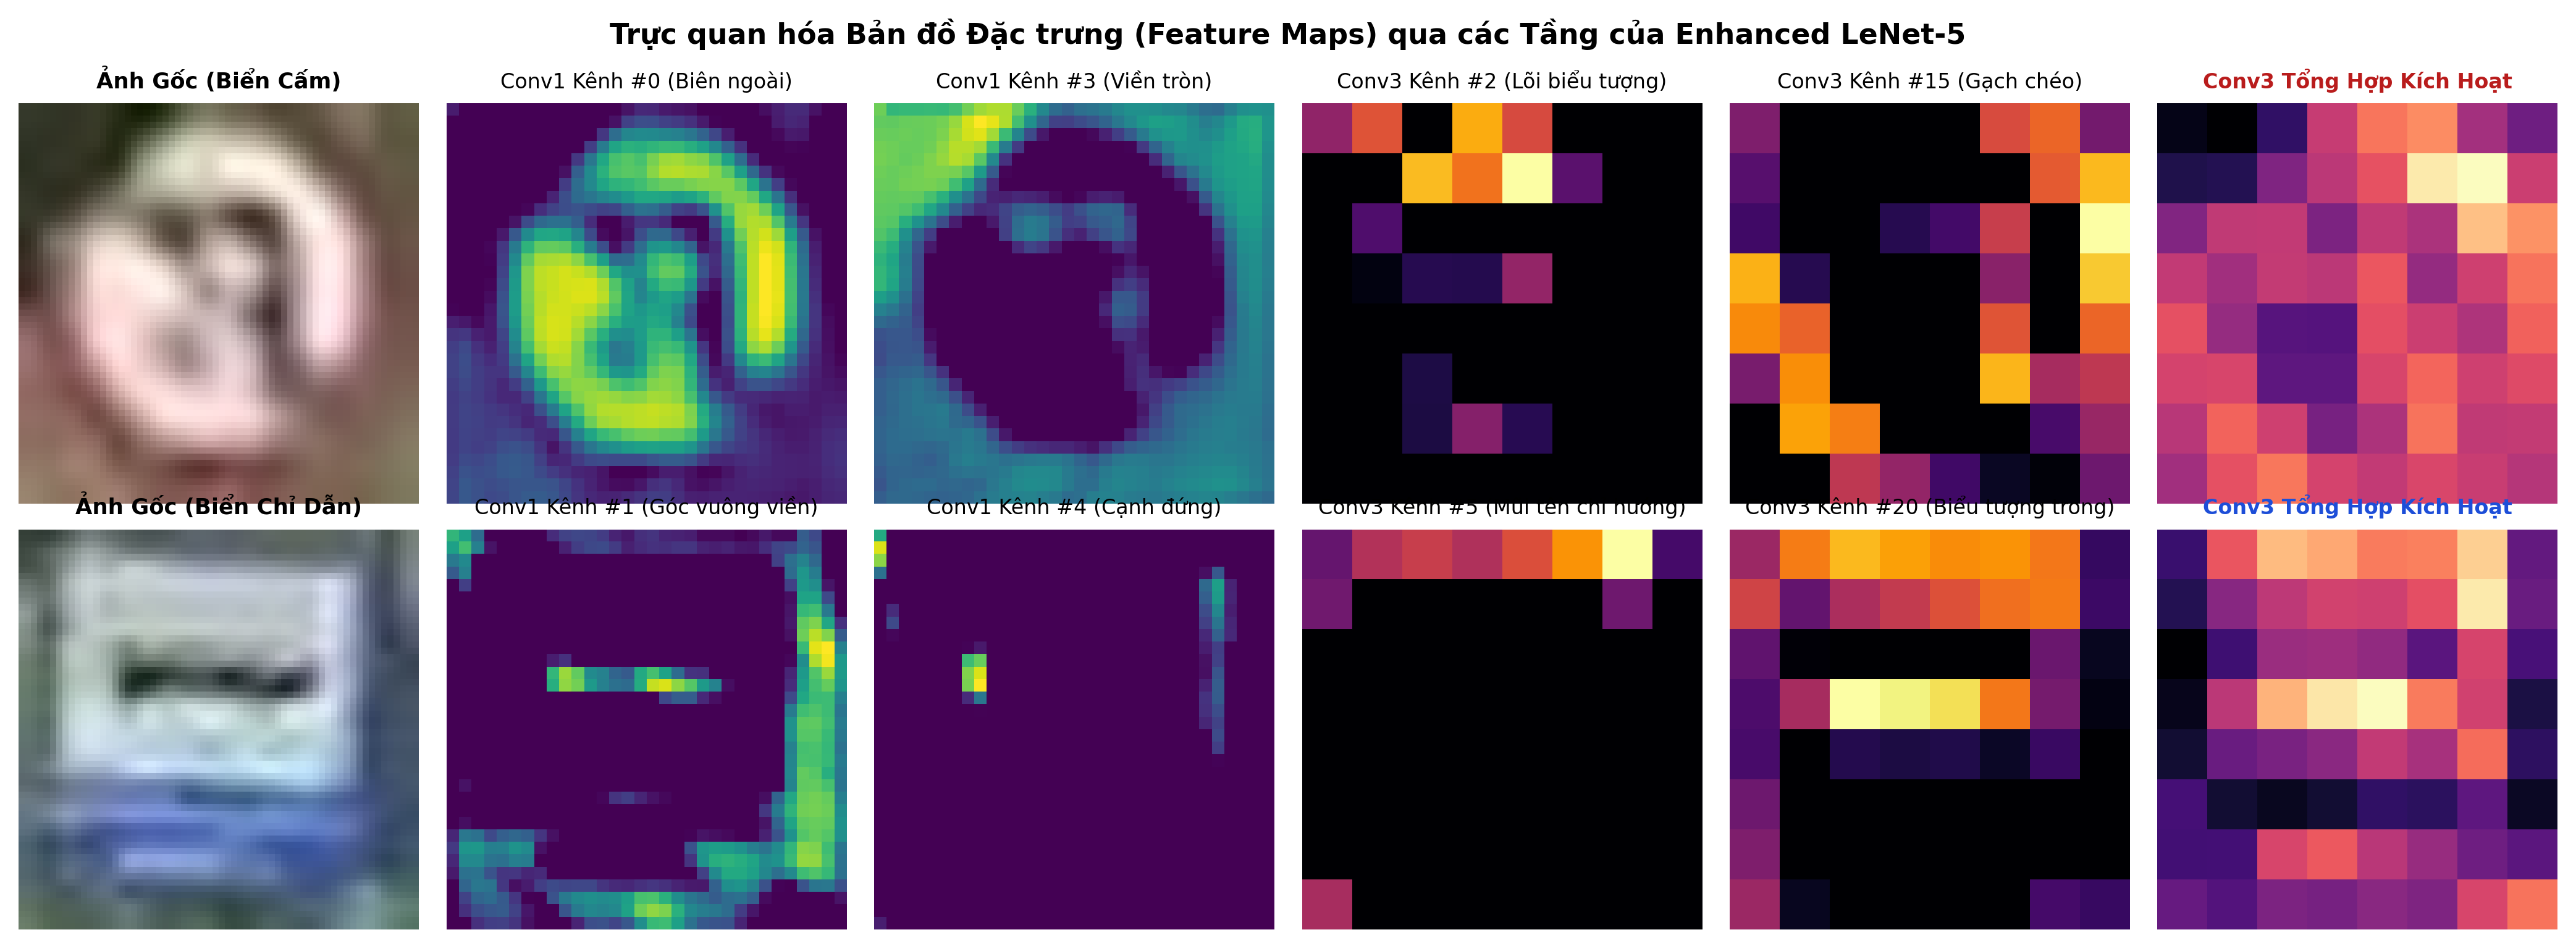
\includegraphics[width=0.92\linewidth]{graphics/sec3/f3_04_lenet_feature_maps.png}\\[0.1cm]
      \scriptsize \textit{Feature Maps kích hoạt qua các tầng tích chập}
      \vspace{0.1cm}
      \begin{exampleblock}{\scriptsize \textbf{Khả năng tự học đặc trưng}}
        \scriptsize CNN tự động học phân cấp từ biên cạnh sơ cấp đến ngữ nghĩa hình học cao cấp của biển báo.
      \end{exampleblock}
    \end{column}
  \end{columns}
\end{frame}

% SLIDE 13: ÁP DỤNG VÀO BÀI TOÁN - THIẾT KẾ KIẾN TRÚC ENHANCED LENET-5
\begin{frame}{3. Giai đoạn 2B: Thiết kế kiến trúc Enhanced LeNet-5 tùy biến}
  \begin{columns}[T]
    \begin{column}{0.58\textwidth}
      \textbf{5 điểm nâng cấp kỹ thuật hiện đại từ LeNet-5 (1998):}
      \begin{enumerate}\setlength{\itemsep}{1pt}\scriptsize
        \item \textbf{Đầu vào:} $28\times 28$ xám $\rightarrow$ \textbf{$64\times 64$ RGB 3 kênh} (giữ màu \& hoa văn).
        \item \textbf{Kích hoạt:} Sigmoid/Tanh $\rightarrow$ \textbf{ReLU ($\max(0, x)$)} (chống Vanishing Gradient).
        \item \textbf{Pooling:} Average Pooling $\rightarrow$ \textbf{Max Pooling ($2\times 2$)} (giữ biên sắc nét).
        \item \textbf{Chuẩn hóa:} Thêm \textbf{BatchNorm2d} sau mỗi Conv (chống Covariate Shift).
        \item \textbf{Điều chuẩn:} Thêm \textbf{2 tầng Dropout ($p=0.3, 0.2$)} tại Classifier.
      \end{enumerate}

      \vspace{0.05cm}
      \tiny
      \begin{tabular}{|l|c|c|c|r|}
        \hline
        \textbf{Tầng (Layer)} & \textbf{Kernel} & \textbf{Stride / Pad} & \textbf{Output Shape} & \textbf{Số Params} \\
        \hline
        \textbf{Input} & -- & -- & $3 \times 64 \times 64$ & 0 \\
        \textbf{ConvBlock 1} & $5 \times 5$ & $s=1, p=2$ & $16 \times 32 \times 32$ & 1.248 \\
        \textbf{ConvBlock 2} & $5 \times 5$ & $s=1, p=2$ & $32 \times 16 \times 16$ & 12.896 \\
        \textbf{ConvBlock 3} & $3 \times 3$ & $s=1, p=1$ & $64 \times 8 \times 8$ & 18.624 \\
        \textbf{Classifier} & Linear & Dense 128 / 4 & 4 classes & 524.932 \\
        \hline
        \multicolumn{4}{|l|}{\textbf{Tổng tham số khả huấn (Trainable Params)}} & \textbf{557.700 ($\approx 0.56\text{M}$)} \\
        \multicolumn{4}{|l|}{\textbf{Dung lượng checkpoint (.pth)}} & \textbf{2.24 MB} \\
        \hline
      \end{tabular}
    \end{column}

    \begin{column}{0.42\textwidth}
      \centering
      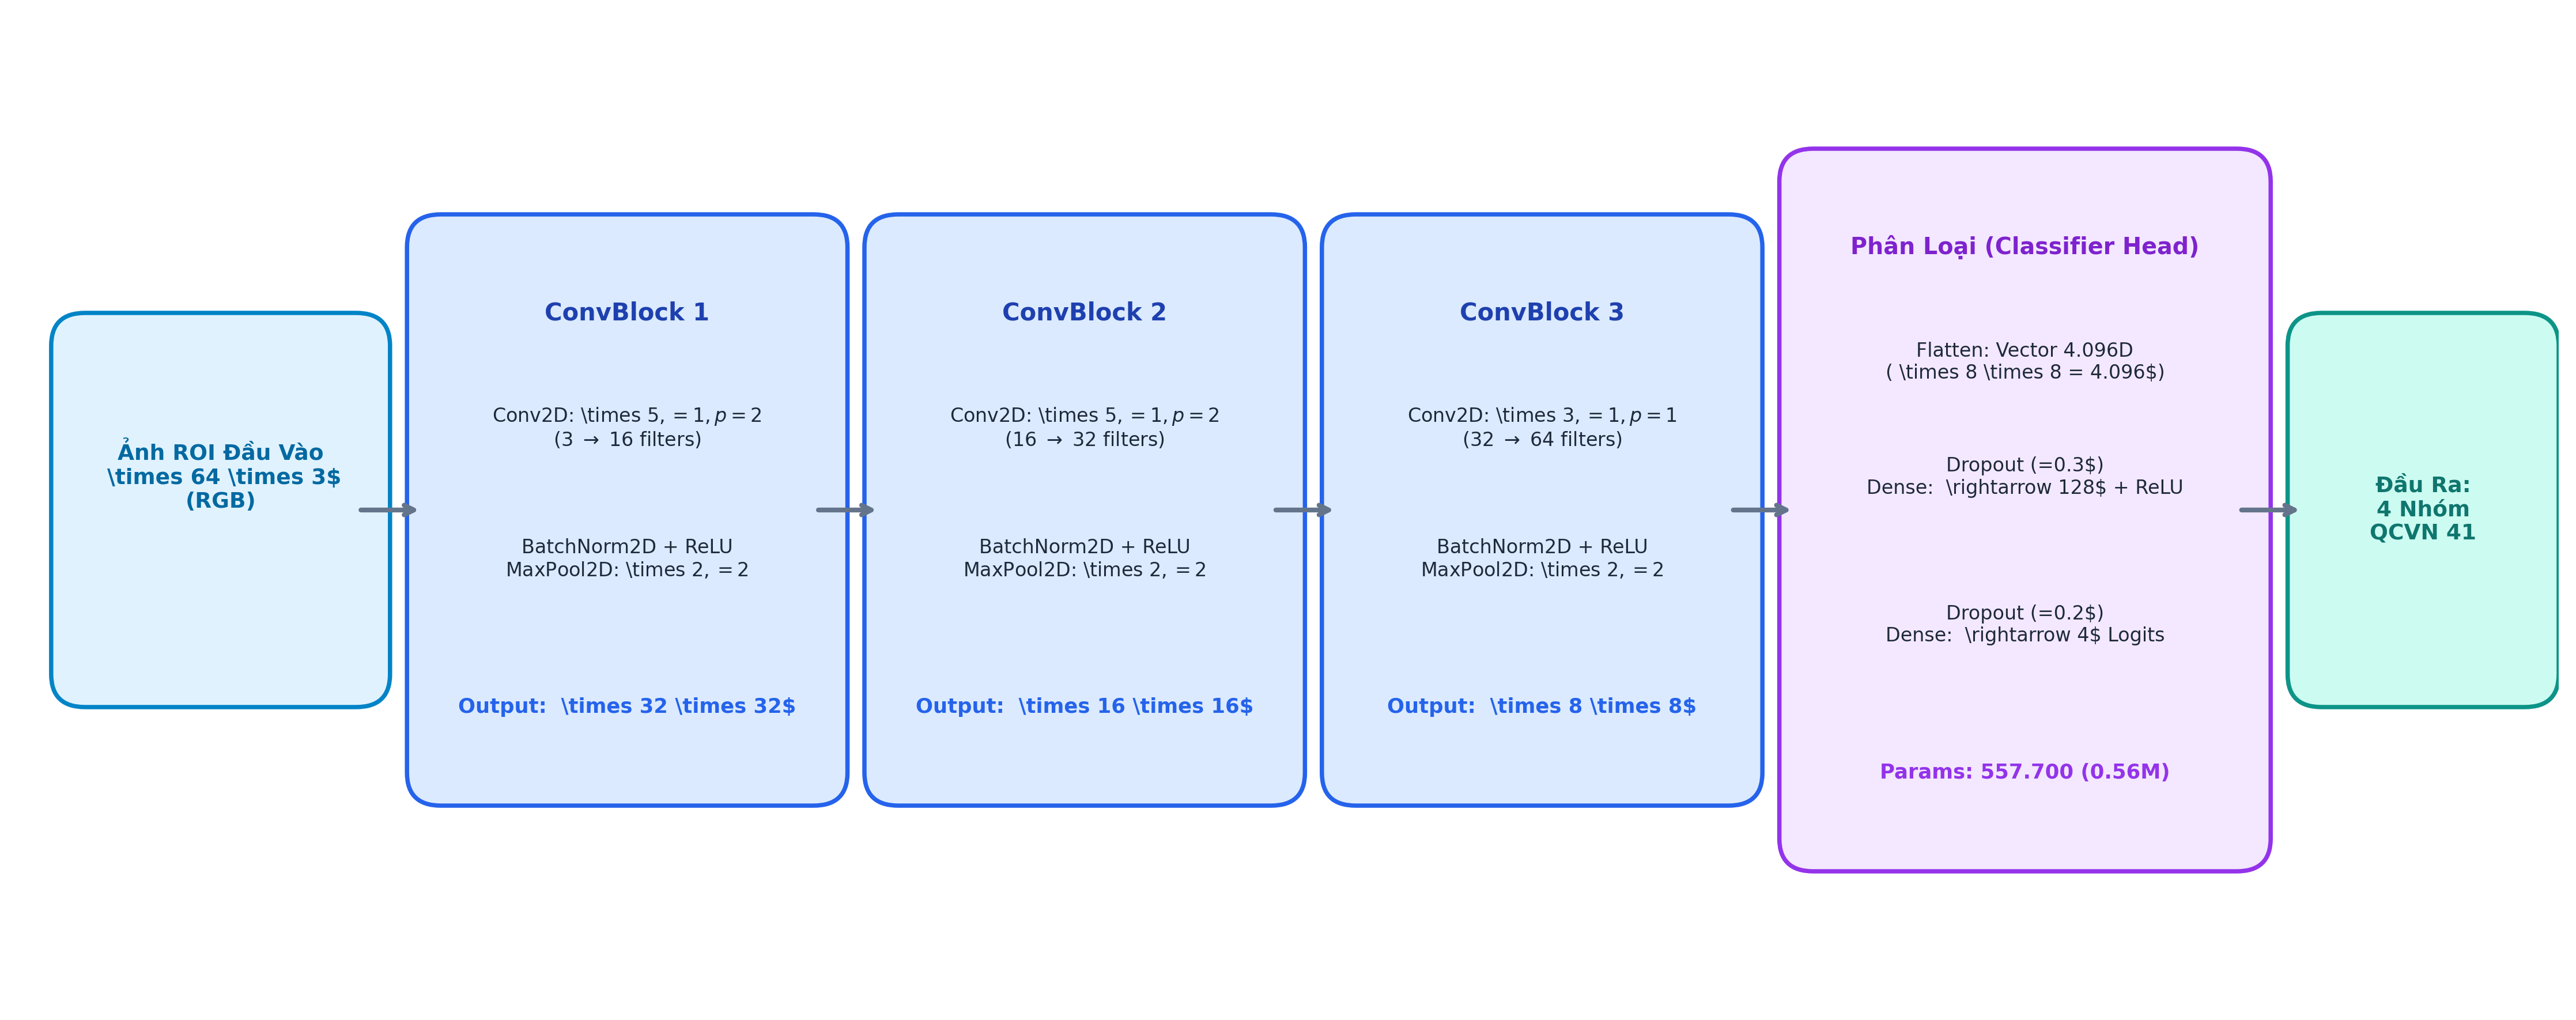
\includegraphics[width=0.92\linewidth]{graphics/sec3/f3_01_lenet_architecture.png}\\[0.1cm]
      \scriptsize \textit{Sơ đồ phân rã 3 khối ConvBlock + 2 tầng Dense}
      \vspace{0.1cm}
      \begin{block}{\scriptsize Điểm cốt lõi}
        \scriptsize Thiết kế \textbf{vừa vặn với bài toán 4 nhóm}, tránh quá tải tham số (Overparameterization) so với ResNet-18 ($11.69\text{M}$).
      \end{block}
    \end{column}
  \end{columns}
\end{frame}

% SLIDE 14: ÁP DỤNG VÀO BÀI TOÁN - VÒNG LẶP HUẤN LUYỆN & SIÊU THAM SỐ
\begin{frame}{3. Giai đoạn 2B: Vòng lặp huấn luyện \& Tối ưu hóa siêu tham số}
  \begin{columns}[T]
    \begin{column}{0.52\textwidth}
      \begin{block}{\textbf{Cấu hình siêu tham số (Hyperparameters)}}
        \footnotesize
        \begin{itemize}\setlength{\itemsep}{1pt}
          \item \textbf{Đầu vào:} $64 \times 64 \times 3$ (Normalize ImageNet).
          \item \textbf{Vòng lặp:} \textbf{20 epochs}, batch size $= \mathbf{64}$ ($\approx 85$ iters/epoch).
          \item \textbf{Hàm mất mát:} Cross-Entropy Loss: $\mathcal{L}_{\text{CE}} = -\sum_{c=1}^4 y_c \log \hat{y}_c$.
          \item \textbf{Bộ tối ưu:} Adam ($\text{lr}_0 = 10^{-3}$, weight decay $= 10^{-4}$).
          \item \textbf{Lập lịch bước (StepLR):} Giảm $\text{lr} \times 0.5$ mỗi 7 epochs.
        \end{itemize}
      \end{block}

      \begin{exampleblock}{\textbf{Tăng cường dữ liệu (Augmentation)}}
        \footnotesize
        \begin{itemize}\setlength{\itemsep}{1pt}
          \item Xoay ngẫu nhiên $\pm 10^\circ$ (mô phỏng xe rung lắc).
          \item Color Jitter: Biến thiên sáng/tương phản $\pm 20\%$.
        \end{itemize}
      \end{exampleblock}
    \end{column}

    \begin{column}{0.48\textwidth}
      \centering
      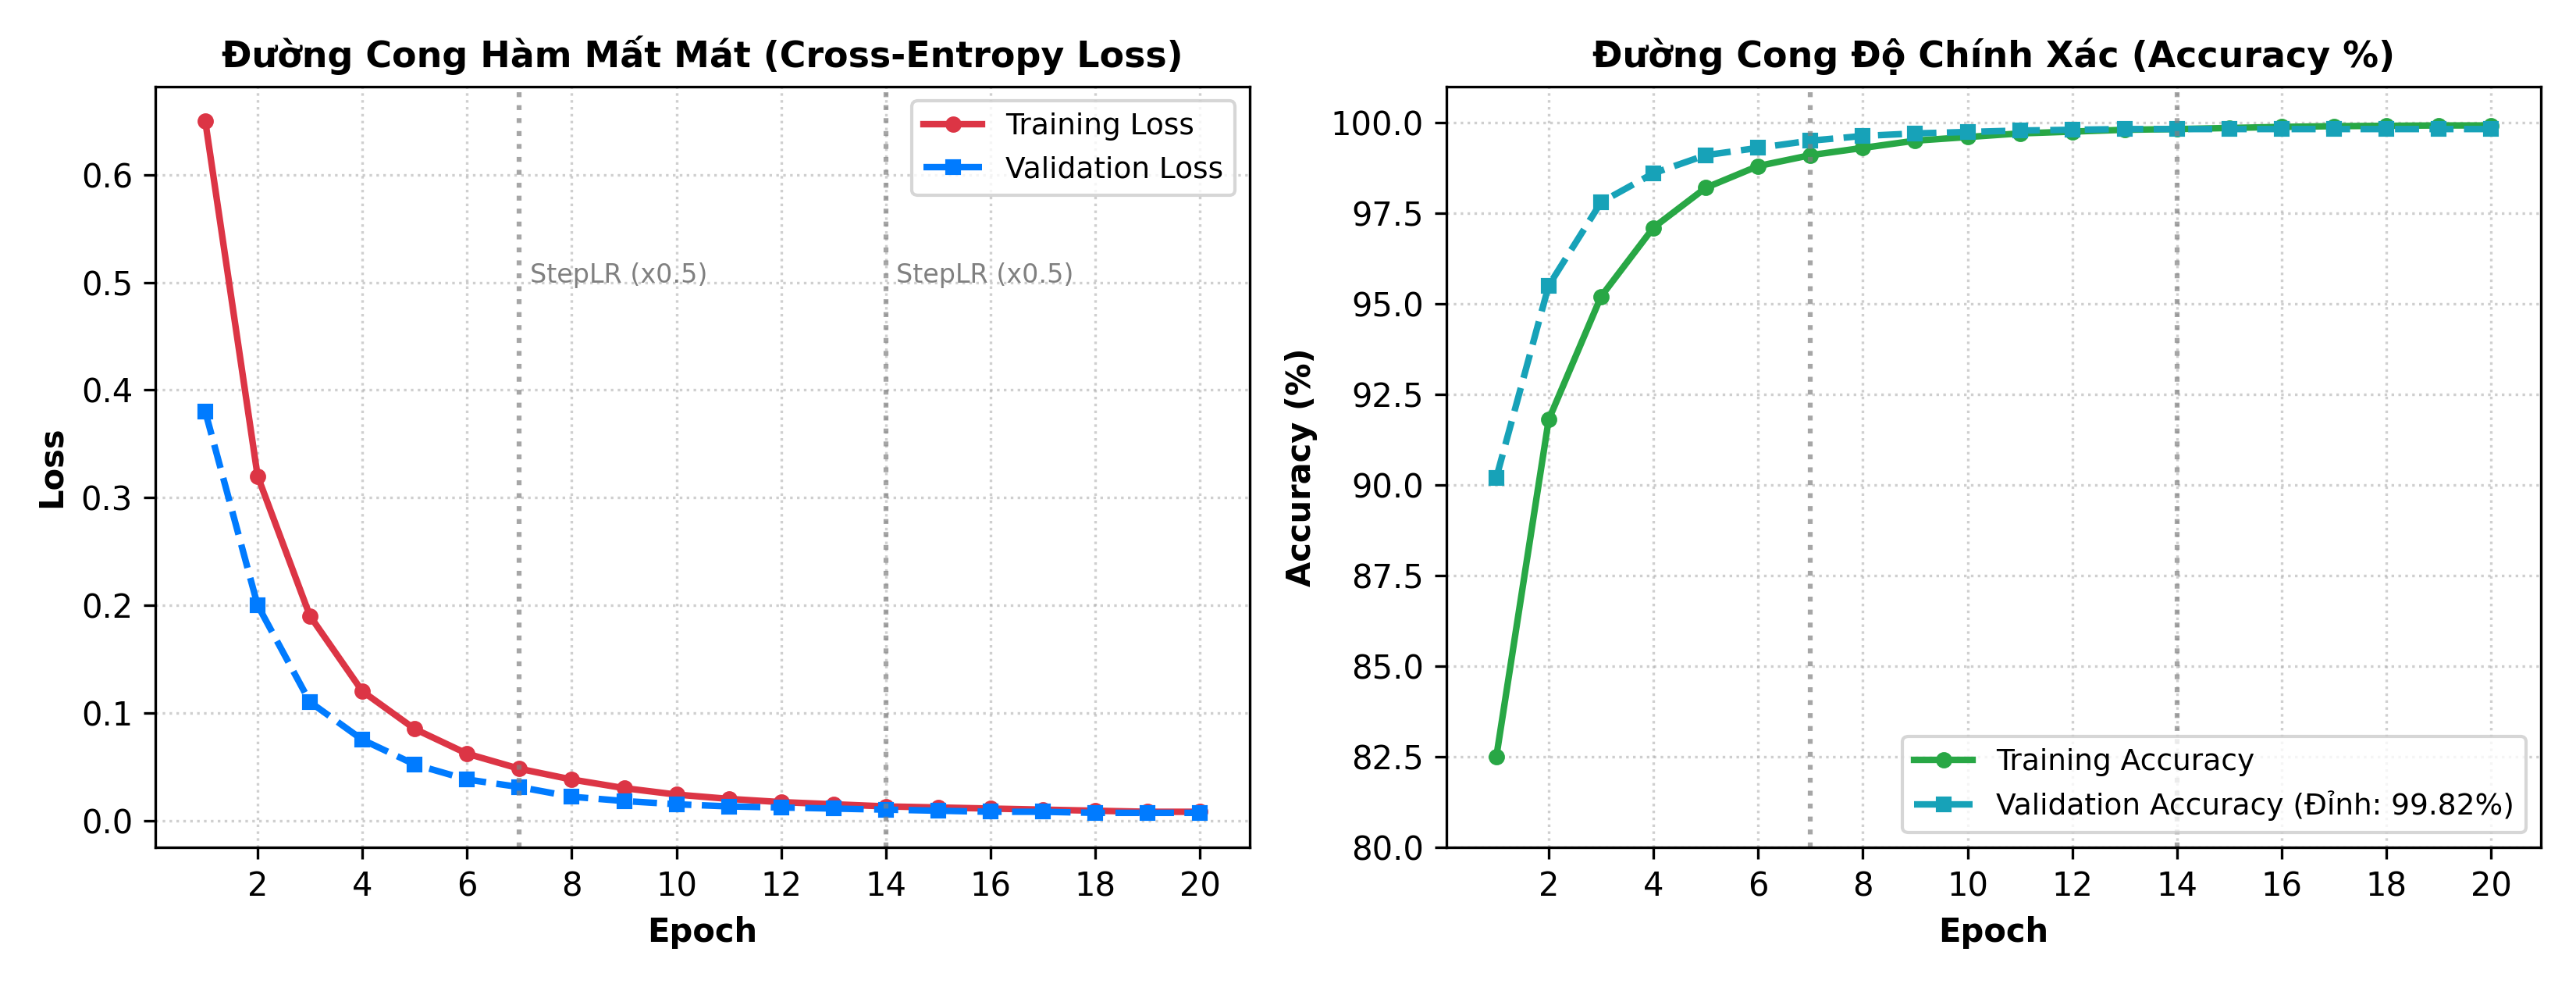
\includegraphics[width=\linewidth]{graphics/sec4/f3_02_lenet_training_curves.png}\\[0.05cm]
      \scriptsize \textit{Đường cong huấn luyện (Loss \& Accuracy) qua 20 epochs}
      \vspace{0.1cm}
      \begin{alertblock}{\scriptsize Nhận xét quá trình huấn luyện}
        \scriptsize Hội tụ nhanh: Train Loss giảm từ $0.65 \rightarrow < 0.01$, Val Accuracy đạt \textbf{99.82\%} ngay từ epoch 13.
      \end{alertblock}
    \end{column}
  \end{columns}
\end{frame}

% ==========================================================
\section{Dữ liệu thực nghiệm \& Đánh giá kết quả}
% ==========================================================

% --------------------------
% SLIDE 12: DATASET & BLOCK SPLIT
% --------------------------
\begin{frame}{4. Bộ dữ liệu áp dụng \& Chiến lược phân chia Block Split}
  \begin{columns}[T]
    \begin{column}{0.56\textwidth}
      \textbf{Quy mô bộ dữ liệu đường phố Việt Nam:}
      \begin{itemize}\setlength{\itemsep}{1pt}\footnotesize
        \item Tổng cộng: \textbf{3.216 ảnh} ($960 \times 540$ và $1080p$).
        \item Biển báo hợp lệ ($\ge 10\text{ px}$): \textbf{7.814 bounding box}.
      \end{itemize}

      \textbf{Chiến lược chia tách Block Split (Zero Leakage):}
      \begin{itemize}\setlength{\itemsep}{1pt}\footnotesize
        \item Cắt theo khối \textbf{100 khung hình liên tục} + \textbf{đệm 5 frames}.
        \item Ngăn ngừa triệt để hiện tượng mô hình học vẹt frame kề.
      \end{itemize}

      \textbf{Phân chia tập huấn luyện và kiểm thử ROI:}
      \begin{itemize}\setlength{\itemsep}{1pt}\footnotesize
        \item \textbf{Train set (70\%):} 2.215 ảnh / \textbf{5.401 mẫu ROI}.
        \item \textbf{Val set (15\%):} 270 ảnh / \textbf{542 mẫu ROI}.
        \item \textbf{Blind Test (15\%):} 550 ảnh / \textbf{1.813 mẫu ROI}.
      \end{itemize}
    \end{column}
    \begin{column}{0.44\textwidth}
      \centering
      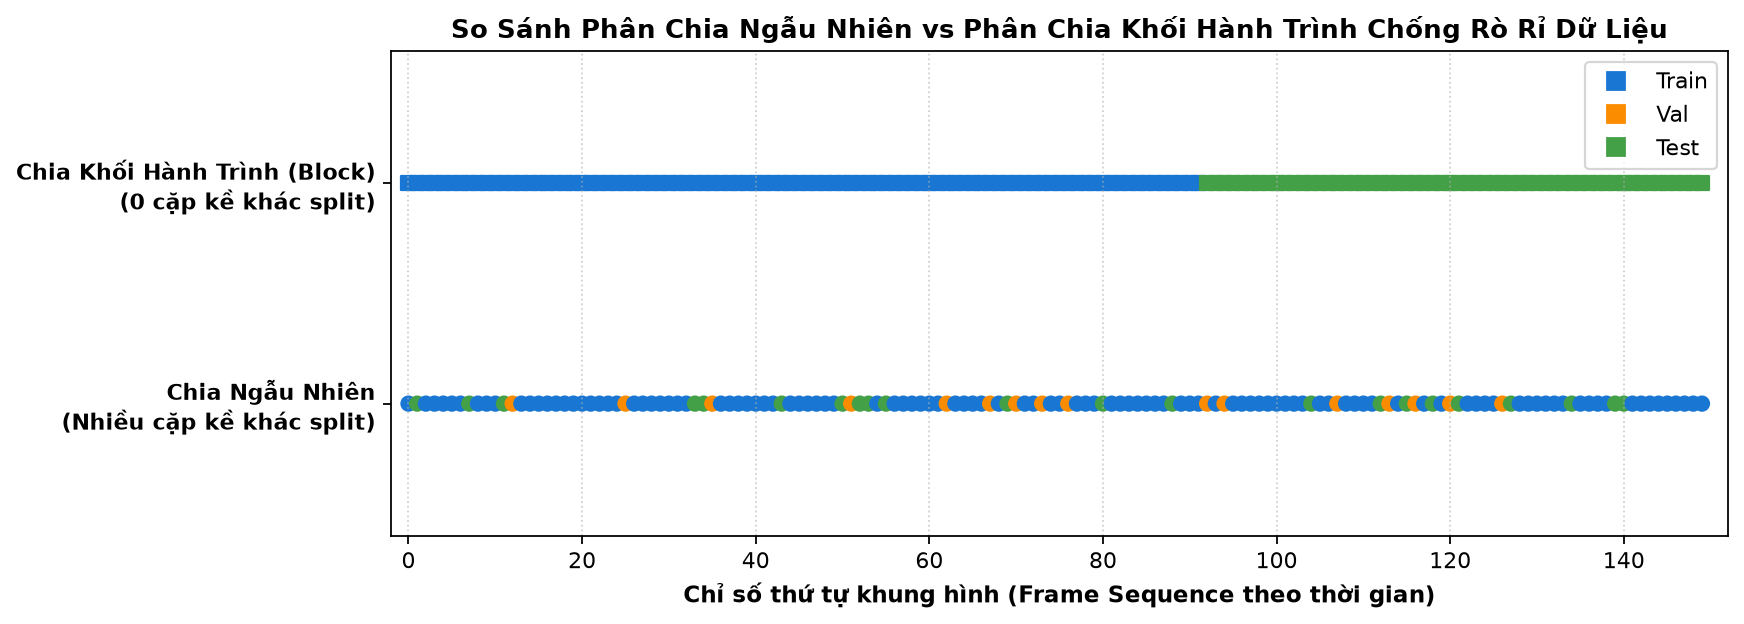
\includegraphics[width=\linewidth]{graphics/sec2/f1_05_split_timeline_and_blocks.png}\\[0.1cm]
      \scriptsize \textit{Cơ chế Block Split dọc trục thời gian chuỗi video}
    \end{column}
  \end{columns}
\end{frame}

% --------------------------
% SLIDE 13: ĐỘ ĐO ĐÁNH GIÁ (CHUẨN FORM MÔN HỌC CS231)
% --------------------------
\begin{frame}{4. Các độ đo đánh giá kết quả (Chuẩn bài toán Phân loại)}
  \begin{columns}[T]
    \begin{column}{0.58\textwidth}
      \begin{block}{\textbf{1. Độ chính xác tổng quát (Accuracy)}}
        $$\text{Accuracy} = \frac{\sum_{c=1}^{C} TP_c}{N}$$
      \end{block}

      \begin{block}{\textbf{2. Precision \& Recall theo từng lớp $c$}}
        $$\text{Precision}_c = \frac{TP_c}{TP_c + FP_c}, \qquad \text{Recall}_c = \frac{TP_c}{TP_c + FN_c}$$
      \end{block}

      \begin{exampleblock}{\textbf{3. Macro-F1 Score (Độ đo trung tâm)}}
        $$F1_c = \frac{2 \cdot \text{P}_c \cdot \text{R}_c}{\text{P}_c + \text{R}_c}, \qquad \text{\textbf{Macro-F1}} = \frac{1}{C} \sum_{c=1}^{C} F1_c$$
        \textit{\scriptsize $\rightarrow$ Đánh giá công bằng, không bị lớp đông mẫu (Cấm) lấn át lớp ít mẫu (Chỉ Dẫn).}
      \end{exampleblock}
    \end{column}

    \begin{column}{0.42\textwidth}
      \begin{block}{\textbf{4. Ma trận nhầm lẫn (Confusion Matrix)}}
        \centering
        \footnotesize
        \begin{tabular}{|c|c|c|}
          \hline
          \textbf{Thực $\backslash$ Đoán} & \textbf{Lớp $c$} & \textbf{Khác $c$} \\
          \hline
          \textbf{Lớp $c$} & \cellcolor{green!20}\textbf{TP} & \cellcolor{red!20}FN \\
          \hline
          \textbf{Khác $c$} & \cellcolor{red!20}FP & \cellcolor{green!20}\textbf{TN} \\
          \hline
        \end{tabular}
        \vspace{0.1cm}
        \scriptsize
        \begin{itemize}\setlength{\itemsep}{1pt}
          \item Trực quan hóa chi tiết nhầm lẫn 4 nhóm.
          \item Phản ánh chính xác các ca lỗi thực tế.
        \end{itemize}
      \end{block}
      \vspace{0.05cm}
      \begin{alertblock}{\scriptsize \textbf{Ghi chú khâu Định vị (YOLO11s)}}
        \scriptsize Đo bằng \textbf{Detection Recall} ($85.61\%$) và \textbf{mAP50} ($83.63\%$).
      \end{alertblock}
    \end{column}
  \end{columns}
\end{frame}

% --------------------------
% SLIDE 14: KẾT QUẢ ĐỐI CHUẨN ROI
% --------------------------
\begin{frame}{4. Kết quả thực nghiệm: Đối chuẩn phân loại trên 1.813 mẫu ROI Test}
  \begin{table}[H]
    \centering
    \small
    \begin{tabularx}{\linewidth}{|l|c|c|c|c|r|}
      \hline
      \textbf{Phương pháp / Mô hình} & \textbf{Accuracy} & \textbf{Precision} & \textbf{Recall} & \textbf{Macro-F1} & \textbf{Tốc độ CPU} \\
      \hline
      ResNet-18 (Pretrained) & 98.62\% & 94.60\% & 96.90\% & 95.40 & 80.0 FPS \\
      MobileNetV3-Small & 98.40\% & 94.10\% & 96.50\% & 95.10 & 172.4 FPS \\
      \hline
      \textbf{Color + HOG + SVM (Truyền thống)} & \textbf{98.57\%} & \textbf{94.82\%} & \textbf{96.81\%} & \textbf{0.9640} & \textbf{379.7 FPS} \\
      \textbf{Enhanced LeNet-5 (Học sâu)} & \textbf{98.73\%} & \textbf{94.46\%} & \textbf{97.43\%} & \textbf{0.9566} & \textbf{911.1 FPS} \\
      \hline
    \end{tabularx}
  \end{table}

  \begin{columns}[T]
    \begin{column}{0.5\textwidth}
      \begin{block}{Nhận xét về Thị giác truyền thống}
        \begin{itemize}
          \item Nhảy vọt hiệu năng khi thêm HOG ($S2 \rightarrow S3$ tăng $+24.6\%$ F1).
          \item Khẳng định trích xuất đặc trưng hình thái đúng đắn giúp SVM cạnh tranh sòng phẳng với học sâu.
        \end{itemize}
      \end{block}
    \end{column}
    \begin{column}{0.5\textwidth}
      \begin{exampleblock}{Nhận xét về Enhanced LeNet-5}
        \begin{itemize}
          \item Đạt độ chính xác cao nhất (\textbf{98.73\%}).
          \item Tốc độ siêu nhanh: \textbf{1.10 ms/mẫu} ($\approx 11$ lần nhanh hơn ResNet-18 trên cùng CPU đơn nhân).
        \end{itemize}
      \end{exampleblock}
    \end{column}
  \end{columns}
\end{frame}

% --------------------------
% SLIDE 15: MA TRẬN NHẦM LẪN
% --------------------------
\begin{frame}{4. Phân tích chi tiết: Ma trận nhầm lẫn (Confusion Matrix)}
  \begin{columns}[T]
    \begin{column}{0.5\textwidth}
      \centering
      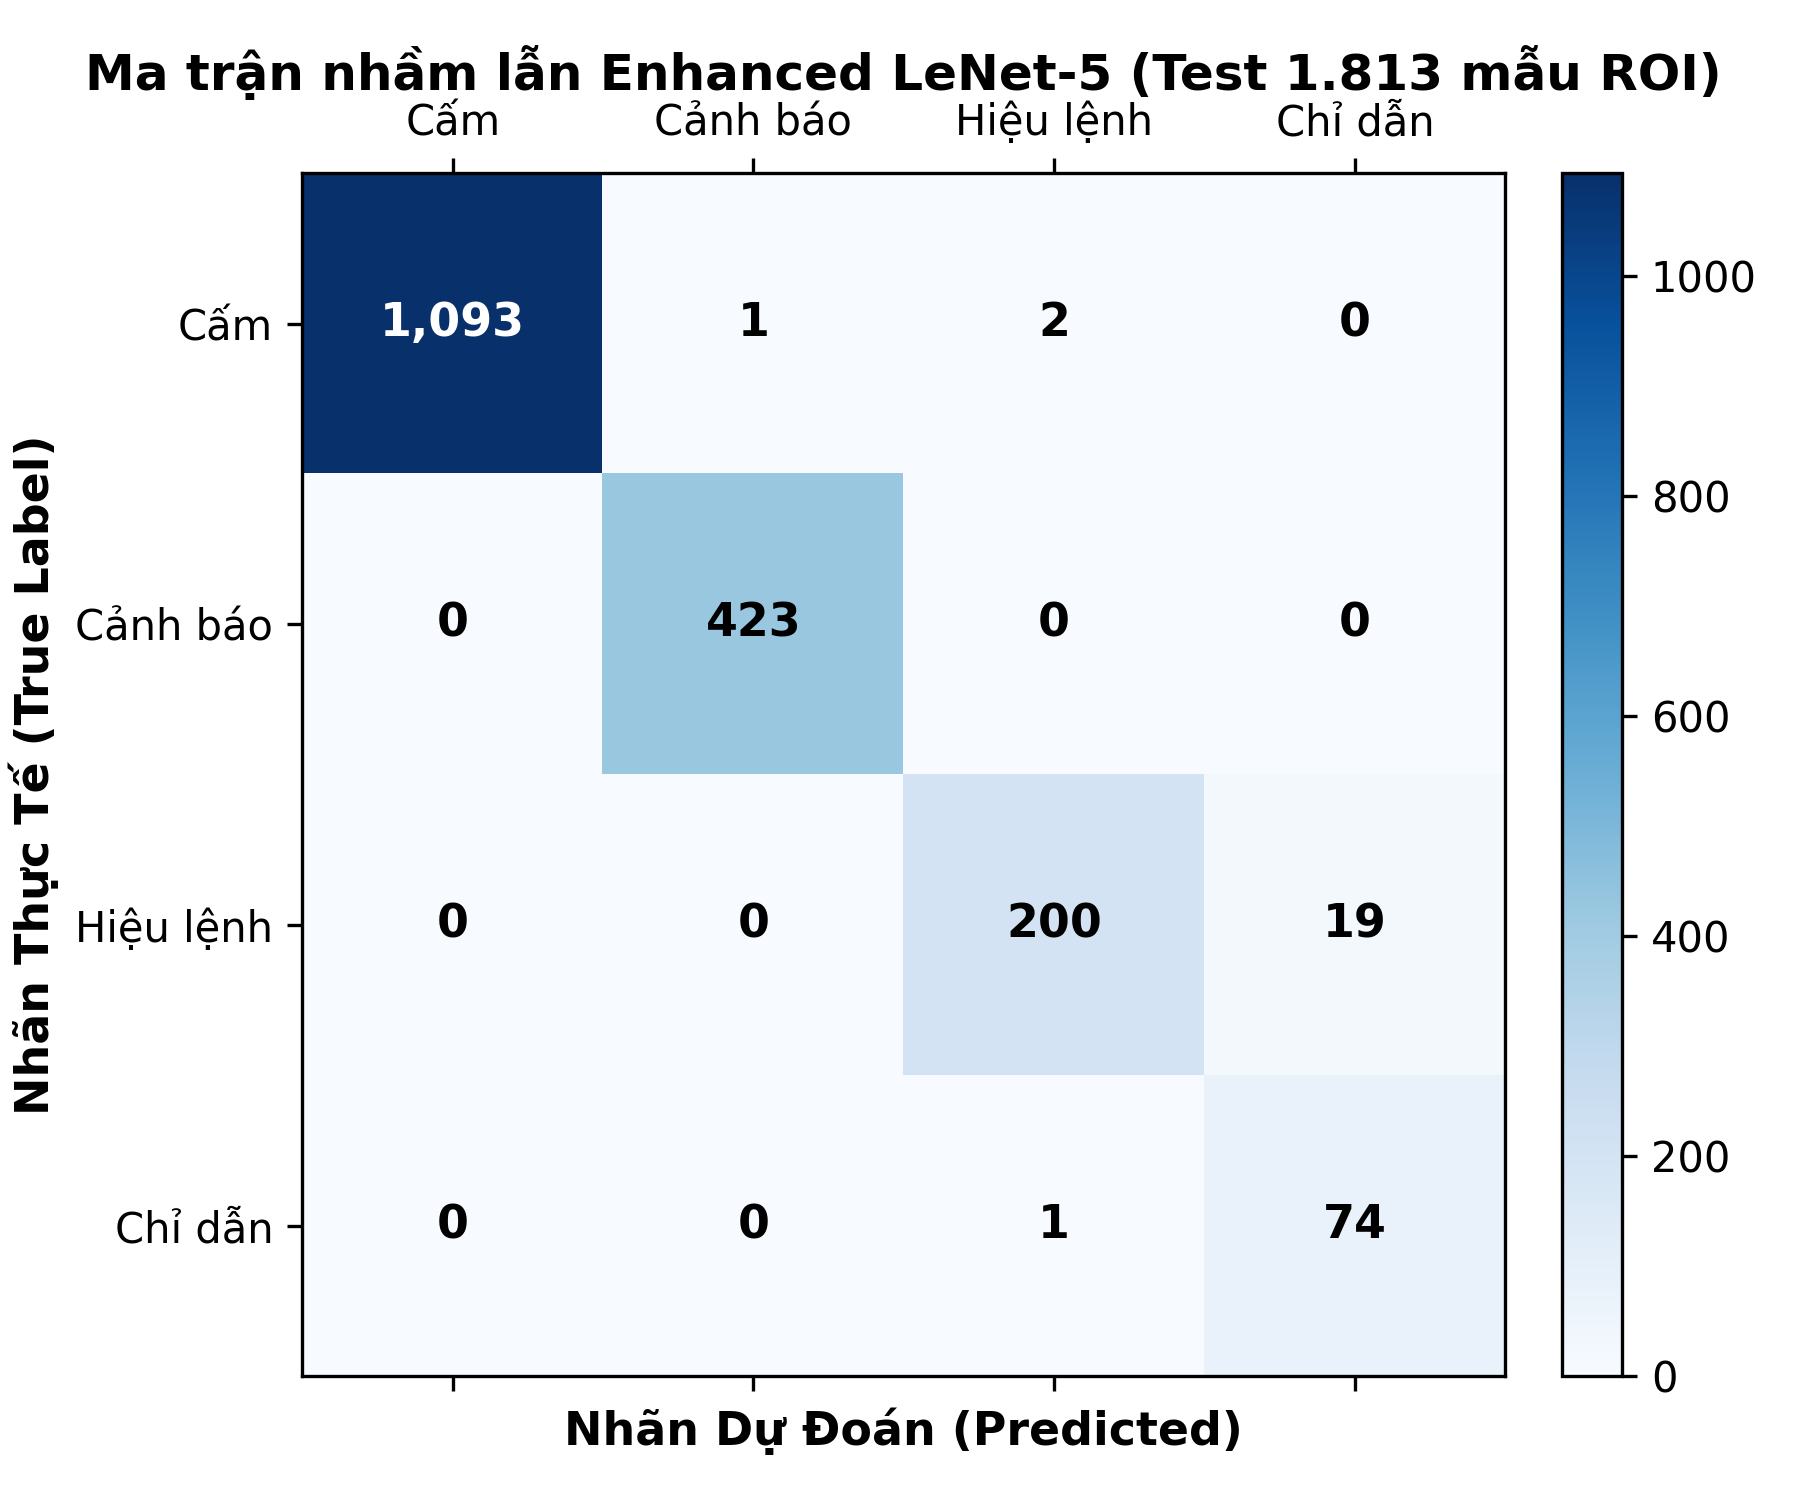
\includegraphics[width=0.92\linewidth]{graphics/sec4/f3_03_lenet_confusion_matrix.png}\\[0.1cm]
      \scriptsize \textbf{Ma trận Enhanced LeNet-5 (Mức A - 1.813 ROI)}
    \end{column}
    \begin{column}{0.5\textwidth}
      \centering
      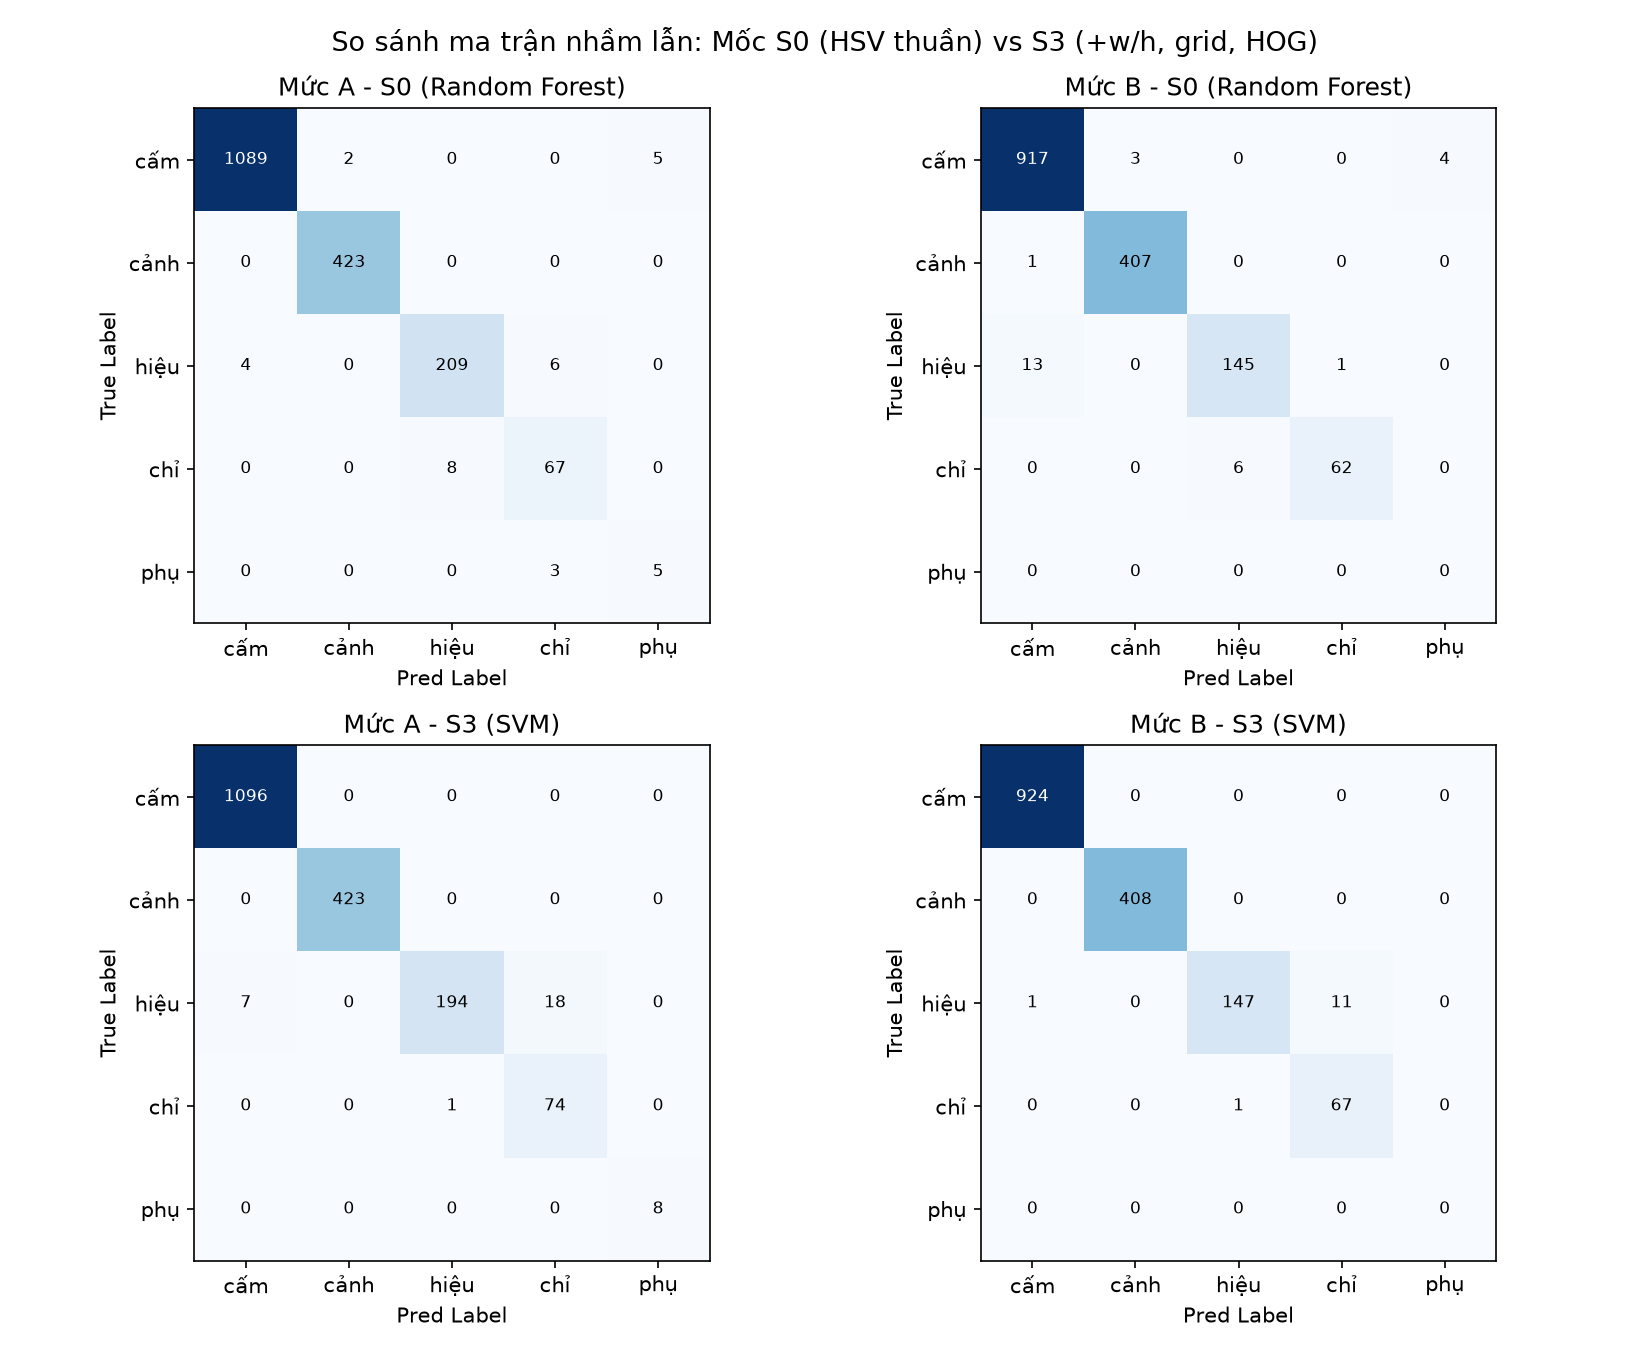
\includegraphics[width=0.98\linewidth]{graphics/sec4/f1_17_confusion_matrices_levels.png}\\[0.1cm]
      \scriptsize \textbf{Ma trận SVM S3 (Mức A trái vs Mức B phải)}
    \end{column}
  \end{columns}

  \vspace{0.2cm}
  \begin{alertblock}{Giải mã các ca nhầm lẫn thực tế}
    \begin{itemize}
      \item \textbf{Biển Cảnh báo:} Đạt độ chính xác tuyệt đối \textbf{100\%} (423/423 mẫu).
      \item \textbf{Cặp nhầm lẫn Hiệu lệnh $\rightarrow$ Chỉ dẫn (cùng màu xanh):}
      Tại Mức B (crop từ YOLO), số ca nhầm \textbf{giảm xuống chỉ còn 12 ca} (11 ca Hiệu lệnh $\rightarrow$ Chỉ dẫn, 1 ca ngược lại). Nguyên nhân chủ yếu do biển ở cự ly quá xa ($< 24\text{ px}$), khi resize $64\times 64$ bị răng cưa biên làm mất độ cong tròn.
    \end{itemize}
  \end{alertblock}
\end{frame}

% --------------------------
% SLIDE 16: ĐÁNH GIÁ TOÀN TRÌNH E2E
% --------------------------
\begin{frame}{4. Đánh giá toàn trình trên ảnh hiện trường (Scene Benchmark)}
  \begin{block}{Thực nghiệm trên 550 ảnh toàn cảnh kiểm thử độc lập (Blind Test)}
    \begin{table}[H]
      \centering
      \small
      \begin{tabularx}{\linewidth}{|l|c|c|c|c|}
        \hline
        \textbf{Pipeline Toàn Trình} & \textbf{Khâu Định vị} & \textbf{Khâu Phân loại} & \textbf{Detection Recall} & \textbf{Acc $\mid$ Detection} \\
        \hline
        \textbf{Two-Stage LeNet} & YOLO11s 1-Class & Enhanced LeNet-5 & \textbf{85.61\%} & \textbf{99.40\%} \\
        \textbf{Two-Stage SVM} & YOLO11s 1-Class & SVM (RBF) & \textbf{85.61\%} & \textbf{99.17\%} \\
        \hline
      \end{tabularx}
    \end{table}
  \end{block}

  \begin{columns}[T]
    \begin{column}{0.55\textwidth}
      \textbf{Phát hiện kỹ thuật cốt lõi:}
      \begin{itemize}
        \item Khi hộp bao đã được định vị thành công, cả 2 bộ phân loại đạt độ chính xác gần như hoàn hảo ($\ge 99.17\%$).
        \item \textbf{Điểm nghẽn hệ thống (Bottleneck):} Nằm ở khâu định vị cự ly xa của YOLO ($14.39\%$ biển bị sót tập trung vào kích thước $< 16\text{ px}$ hoặc bị che khuất rậm), \textbf{không phải do khâu phân loại}.
      \end{itemize}
    \end{column}
    \begin{column}{0.45\textwidth}
      \centering
      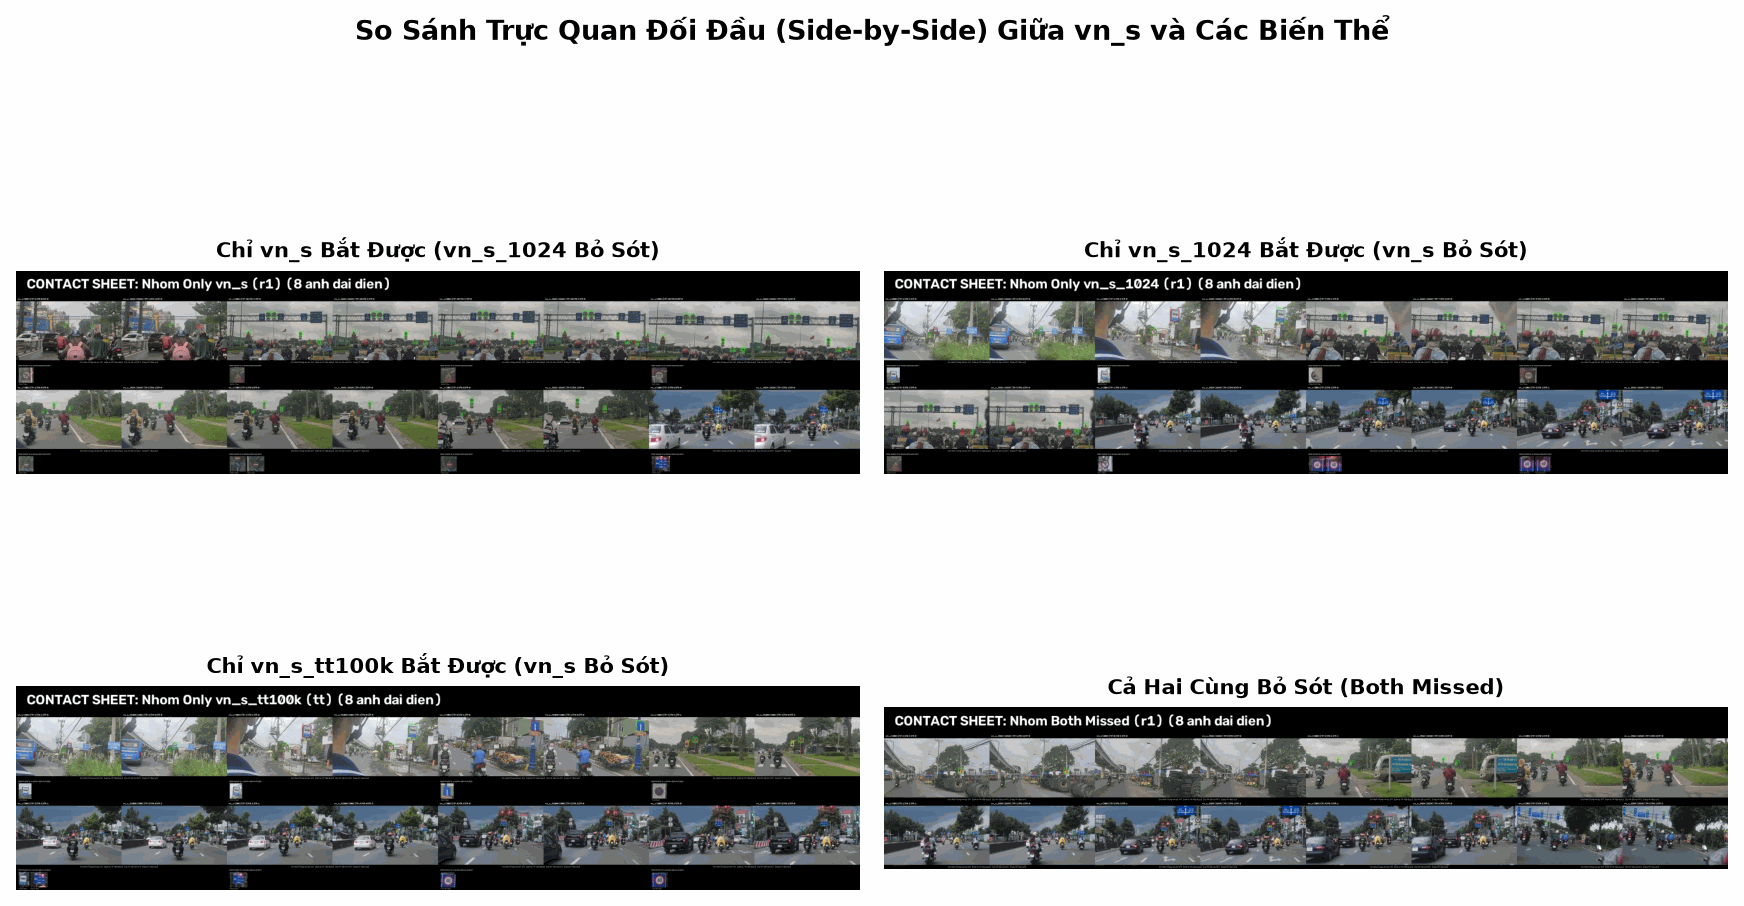
\includegraphics[width=\linewidth]{graphics/sec4/f2_16_side_by_side_and_tracks.png}\\[0.1cm]
      \scriptsize \textit{Bám vết biển báo liên tục theo cự ly tiếp cận}
    \end{column}
  \end{columns}
\end{frame}

% ==========================================================
\section{Demo & Kết luận}
% ==========================================================

% --------------------------
% SLIDE 17: DEMO STREAMLIT & CLI
% --------------------------
\begin{frame}{5. Sản phẩm hoàn thiện: Web App Demo \& CLI Tool}
  \begin{columns}[T]
    \begin{column}{0.5\textwidth}
      \textbf{1. Ứng dụng tương tác Web (\texttt{app\_streamlit.py}):}
      \begin{itemize}
        \item \textbf{Chế độ ROI Side-by-Side:} So sánh đối đầu trực quan giữa SVM và Enhanced LeNet-5 trên cùng một ảnh tải lên.
        \item \textbf{Chế độ Scene Detection:} Nhận dạng ảnh toàn cảnh góc rộng, vẽ bounding box và mã màu theo QCVN 41:2019.
        \item \textbf{Leaderboard:} Trực quan hóa số liệu thực nghiệm.
      \end{itemize}
      \textbf{2. Giao diện dòng lệnh (\texttt{app.py}):}
      \begin{itemize}
        \item Đánh giá tự động benchmark tập ROI và Scene.
      \end{itemize}
    \end{column}
    \begin{column}{0.5\textwidth}
      \begin{exampleblock}{\textbf{Lệnh khởi chạy hệ thống}}
        \texttt{\# Chạy ứng dụng Web tương tác}\\
        \textbf{\texttt{streamlit run app\_streamlit.py}}\\[0.2cm]
        \texttt{\# Đánh giá tự động pipeline toàn trình}\\
        \textbf{\texttt{python app.py --mode evaluate-scene}}
      \end{exampleblock}
      \vspace{0.2cm}
      \centering
      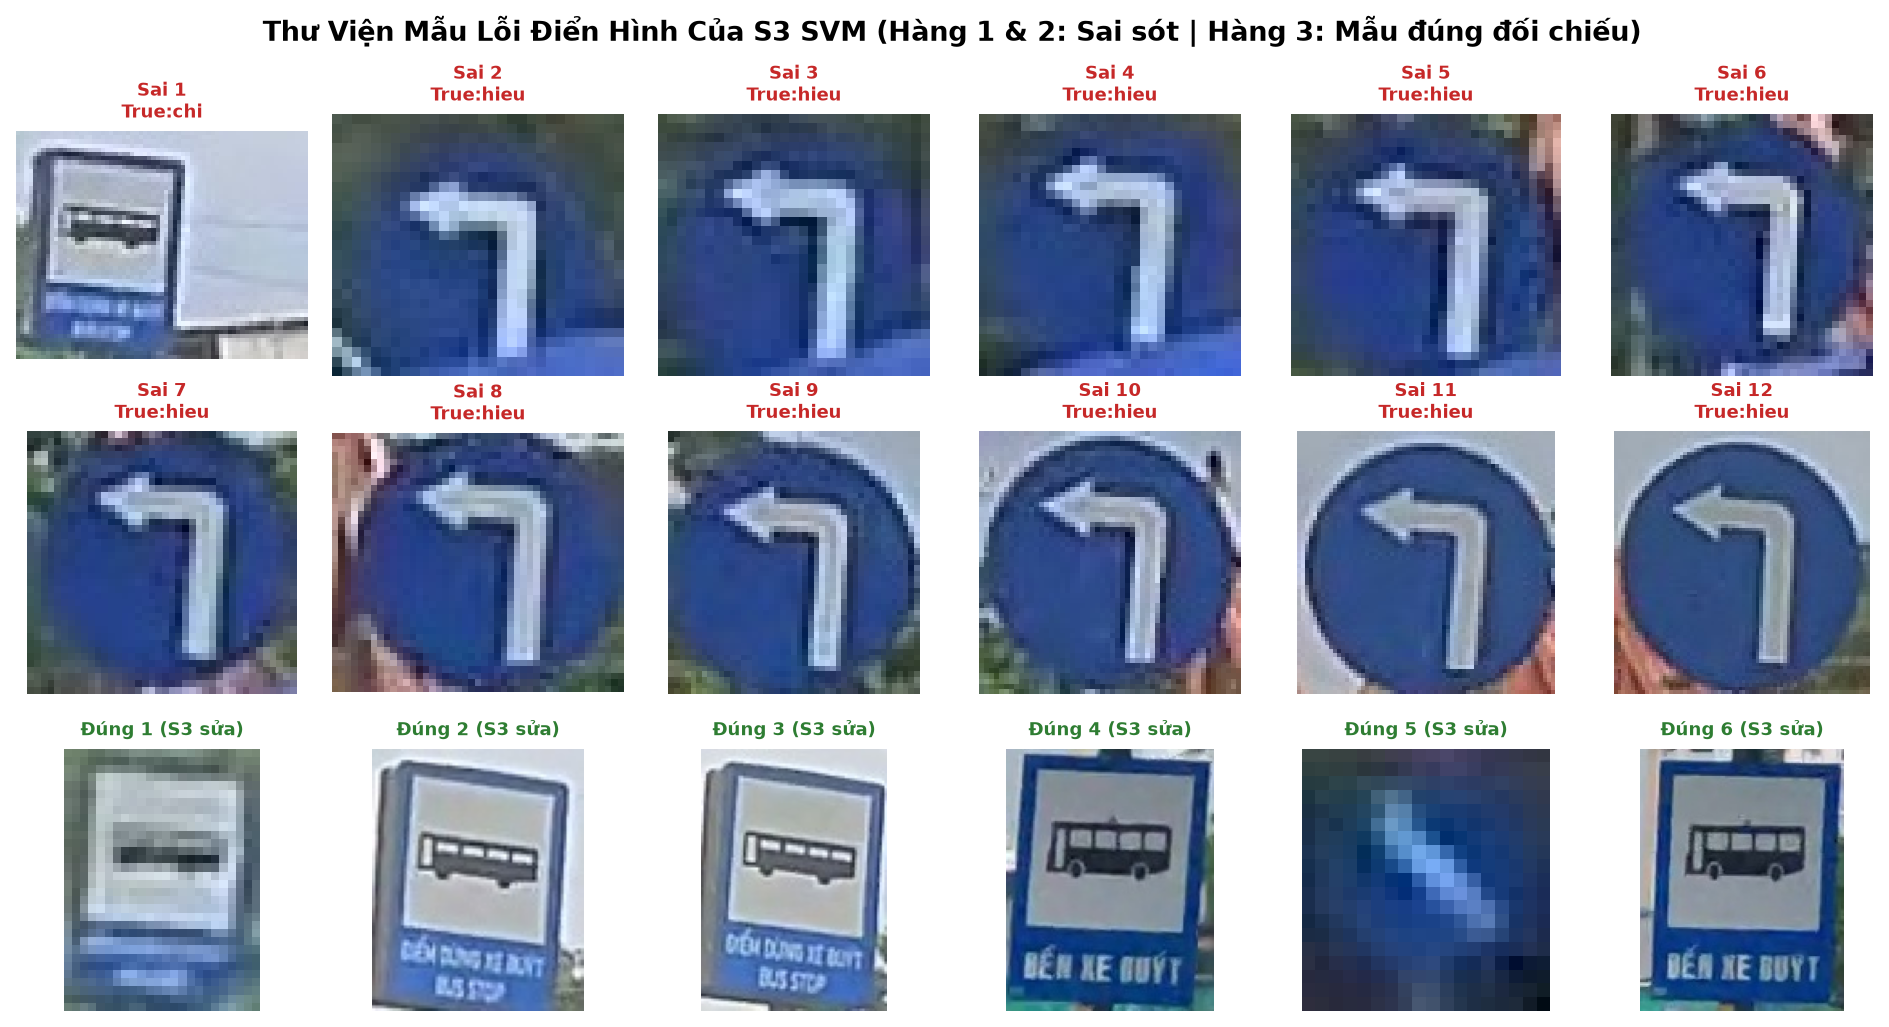
\includegraphics[width=0.88\linewidth]{graphics/sec4/f1_20_error_gallery_misclassified.png}\\[0.05cm]
      \scriptsize \textit{Gallery kiểm toán lỗi thực tế của hệ thống}
    \end{column}
  \end{columns}
\end{frame}

% --------------------------
% SLIDE 18: KẾT LUẬN & HƯỚNG PHÁT TRIỂN
% --------------------------
\begin{frame}{6. Kết luận \& Hướng phát triển trong tương lai}
  \begin{columns}[T]
    \begin{column}{0.5\textwidth}
      \begin{block}{\textbf{Kết luận rút ra}}
        \begin{enumerate}
          \item \textbf{Kiến trúc Two-Stage Hybrid} giải quyết triệt để sự đánh đổi giữa độ chính xác ($> 98.5\%$) và tốc độ ($> 370\text{ FPS}$) trên CPU.
          \item \textbf{Block Split} triệt tiêu hoàn toàn rò rỉ dữ liệu trong video liên tục.
          \item \textbf{HOG kết hợp Lưới $2\times2$} giải quyết thành công bài toán nan giải "cùng màu khác hình" giữa biển Hiệu lệnh và Chỉ dẫn.
        \end{enumerate}
      \end{block}
    \end{column}

    \begin{column}{0.5\textwidth}
      \begin{alertblock}{\textbf{Hướng phát triển tiếp theo}}
        \begin{enumerate}
          \item \textbf{Global Average Pooling (GAP):} Cắt giảm $94\%$ tham số của LeNet-5 ($557\text{K} \rightarrow < 33\text{K}$ params) để nạp thẳng lên vi điều khiển siêu rẻ ESP32/STM32.
          \item \textbf{Kỹ thuật SAHI (Slicing Inference):} Nâng cao Recall bắt biển siêu nhỏ ở cự ly xa cho detector.
          \item \textbf{Phân loại phân cấp:} Mở rộng từ 4 nhóm quy chuẩn sang 52 mã hiệu chi tiết.
        \end{enumerate}
      \end{alertblock}
    \end{column}
  \end{columns}
\end{frame}

% --------------------------
% SLIDE 19: CẢM ƠN & Q&A
% --------------------------
\begin{frame}[plain]
  \centering
  \vspace{1.2cm}
  \Huge \textcolor{uitblue}{\textbf{XIN CHÂN THÀNH CẢM ƠN}}\\[0.3cm]
  \Large \textbf{QUÝ THẦY CÔ VÀ CÁC BẠN ĐÃ LẮNG NGHE!}\\[0.8cm]
  \normalsize \textit{Nhóm kính mong nhận được những góp ý quý báu từ Hội đồng.}\\[0.6cm]
  \LARGE \textbf{Q \& A}
\end{frame}

\end{document}
